%===============================================================
% Template using official colors of Czech Technical University.
% They are defined by new graphical manual - 2017.
% Specially designed for Laboratory of Structure of Biomolecules
% Share and modify as you like. Keep the name of the author.
% It is forbidden to use the template commercially.
% Author: Martin Malý.
% Published: 23.9.2017.
%===============================================================

\documentclass{beamer}
\usepackage[utf8]{inputenc}
\usepackage{ulem}

\usetheme{Madrid}
  
\definecolor{cvut_navy}{HTML}{0065BD}
\definecolor{cvut_blue}{HTML}{6AADE4}
\definecolor{cvut_gray}{HTML}{156570}

\setbeamercolor{section in toc}{fg=black,bg=white}
\setbeamercolor{alerted text}{fg=cvut_blue}
\setbeamercolor*{palette primary}{bg=cvut_navy,fg=gray!20!white}
\setbeamercolor*{palette secondary}{bg=cvut_blue,fg=white}
\setbeamercolor*{palette tertiary}{parent=palette primary}
\setbeamercolor*{palette quaternary}{fg=green,bg=gray!5!white}

\setbeamercolor*{sidebar}{fg=cvut_navy,bg=gray!15!white}


\setbeamercolor{titlelike}{parent=palette primary}
\setbeamercolor{frametitle}{parent=palette primary}

\setbeamercolor*{separation line}{}
\setbeamercolor*{fine separation line}{}

\setbeamertemplate{navigation symbols}{} 

\usepackage{pifont}
\usepackage{tikz}

\usepackage{eqnarray,amsmath}
\usepackage{amsfonts}
\usepackage{amssymb}
\usepackage{graphicx}
\usepackage{lmodern} % pro pismo tucne a zaroven kurziva
\usepackage{bm} % pro pismo tucne a zaroven kurziva
\usepackage{epstopdf}
\usepackage{changepage}
\usepackage{array,booktabs}

% definice makra pro české uvozovky:
\def\bq{\mbox{\kern.1ex\protect\raisebox{-1.3ex}[0pt][0pt]{''}\kern-.1ex}}
\def\eq{\mbox{\kern-.1ex``\kern.1ex}}
\def\ifundefined#1{\expandafter\ifx\csname#1\endcsname\relax }%
\ifundefined{uv}%
        \gdef\uv#1{\bq #1\eq}
\fi
% konec .... použití makra pro psaní český uvozovek: \uv{text uvnitř uvozovek}

%====================================================
%========== DEFINITION OF AUTHORS ETC...=============
%====================================================
\author[by Iulian]{ \textit{de Andreicovici Iulian Florin}}
\institute[UPB]{\large \textbf{Universitatea Politehnica din București}\\ 
\vspace{2mm} FSA \\ IF-1334 }
\title[Inginerie soft]{\textbf{HYPATIA}}
\subtitle{Hybrid Pupil's Analysis Tool for Interactions in Atlas}
\date[Aplicație experimentală.]{\textbf{August, 2022}}

%====================================================
%========== BEGINNING OF DOCUMENT ===================
%====================================================
\begin{document}

\begin{frame}
	\titlepage
	\begin{center}
		
\includegraphics[height=2cm]{files/channels4_profile.jpg}
		
\includegraphics[height=2cm]{files/cern.jpg}
  	
\includegraphics[height=1.5cm]{files/LOGO_HYPATIA_web.png}
	\end{center}
\end{frame}


\logo{
\includegraphics[height=0.5cm]{files/symbol_cvut_plna_samostatna_verze.pdf}}

%.................................................................................
%slide1

\begin{frame}{Ce face HYPATIA pentru noi?}

\underline{\textit{\textbf{În primul rând marcăm ideile de bază:}}}\\
\vspace{0.2cm}
\makebox[1cm]{} \textit{{\textbf{1) \textcolor{blue}{HYPATIA} nu este nimic mai mult decât un simplu tool dedicat procesării cât și analizei evenimentelor provenite din experimentul ATLAS de la LHC;}}}\\
.........................................................................................................\\
\makebox[1cm]{} \textit{\textbf{2) Hypatia permite vizualizarea grafică precum și afișarea particulelor care rezultă din ciocnirile între fasciculele de protoni - sub forma unor amprente/dâre care marchează și interacțiunea fizică dintre ele și straturile detectoare.}}\\
.........................................................................................................\\
\makebox[1cm]{} \textit{\textbf{3) Interfața aplicației este simplă și permite directa exploatare a datelor de output care sunt înregistrate la LHC, având o rezoluție destul de bună în redarea fidelă a semnăturilor anumitor tipuri de particule!}}

\end{frame}
%...............................................................................

%slide2

\begin{frame}{Legătura dintre softul HYPATIA și ATLAS?}

\vspace{-4cm}

 \begin{itemize}
    
 \item[\ding{43}]{\makebox[0.5cm]{} \textbf{Scopul său principal}: urmărirea "tracks-urilor" sau a traiectoriilor particulelor care rezultă din ciocnirile protonilor dar și studiul parametrilor fizici care stau la baza identificării identității lor;}

\end{itemize}      

 \begin{tikzpicture}[overlay, remember picture]
 \node[anchor=center, 
      xshift=-2.7cm, 
      yshift=-1cm] 
     at (current page.center)
     {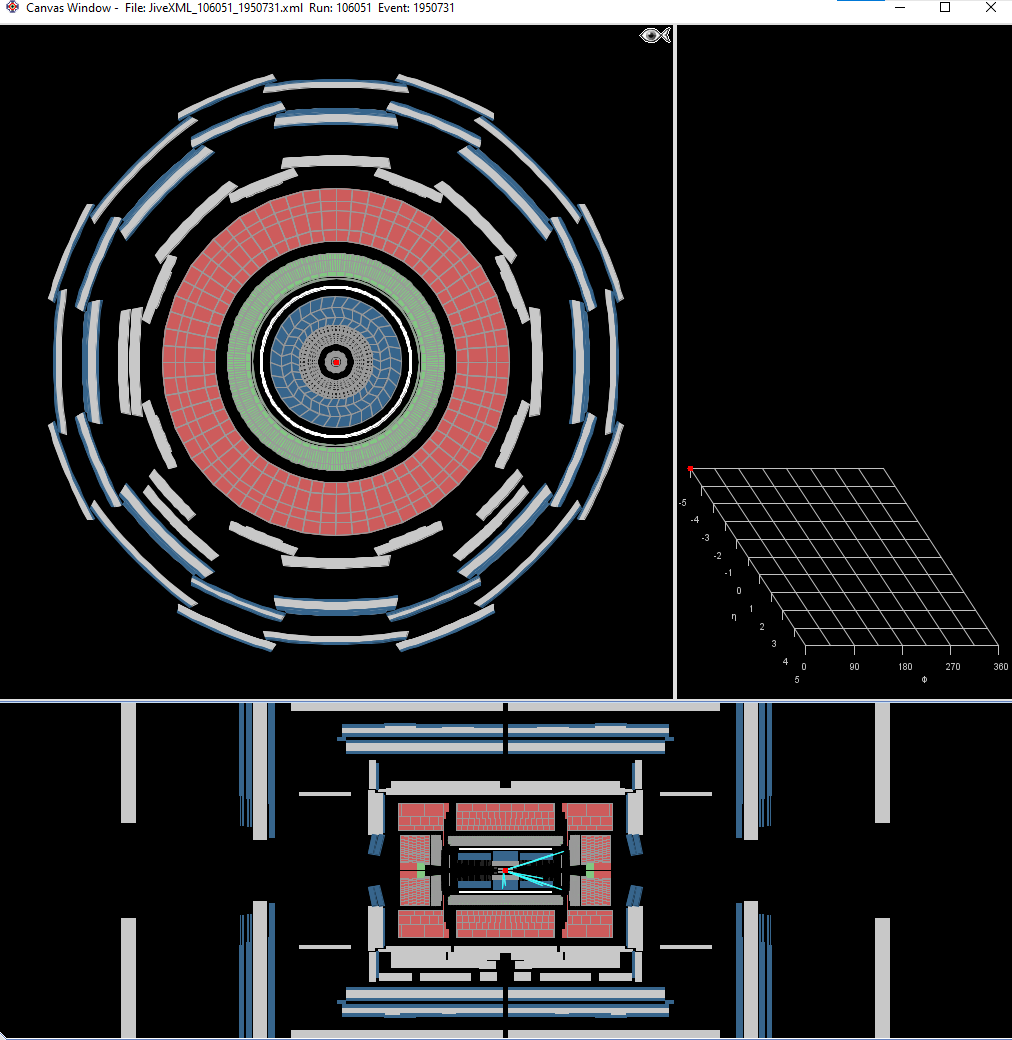
\includegraphics[scale = 0.22]{files/Interfata.png}}; 
 \end{tikzpicture}


  \begin{tikzpicture}[overlay, remember picture]
 \node[anchor=center, 
      xshift=3.5cm, 
      yshift=-1.2cm] 
     at (current page.center)
     {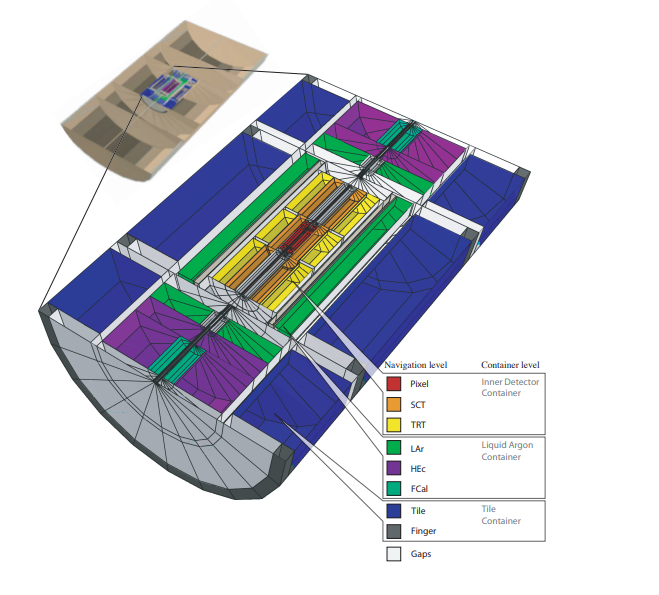
\includegraphics[scale = 0.4]{files/Tota;.png}}; 
 \end{tikzpicture}


\end{frame}

%frame3

\begin{frame}{\textbf{Ce semnifică?}}


 \begin{itemize}
     \small
 \item[\ding{45}]{\makebox[0.5cm]{} \textbf{Fiecare secțiune inelară semnifică un anumit tip de detector - întreaga stratificare este prezentată astfel încât elementele sale să fie ușor de recunoscut;}} \\
  +
  \item[\ding{45}]{\makebox[0.5cm]{} \textbf{"It displays the tracks together with their signature in the different detector parts: the special track detectors, the calorimeters and the large outer muon spectrometer."}}\\
 +
    \item[\ding{45}]{\makebox[0.5cm]{} \textbf{ 
   "Descoperirea" de particule noi se va face prin reconstruirea lor din urmărirea pistelor produselor de dezintegrare!" Manipularea evenimentelor este una selectivă de altfel.}}\\
  +
   \item[\ding{45}]{\makebox[0.5cm]{} \textbf{\textcolor{red}{\textit{ 
   Obiectivele principale ale programului sunt investigarea vizuală și înțelegerea fizicii din spatele evenimentelor reale; \textcolor{blue}{oferă deci informații despre variațiile induse de particule la traversarea detectorilor.}}}}}


\end{itemize}  
\end{frame}

%frame3
\begin{frame}{\textbf{I) REAL Inner Detector:}}
 
 \begin{tikzpicture}[overlay, remember picture]
 \node[anchor=center, 
      xshift=0cm, 
      yshift=-1cm] 
     at (current page.center)
     {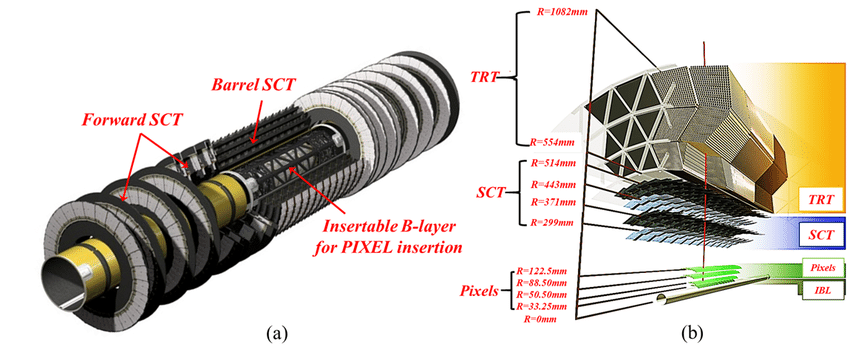
\includegraphics[scale = 0.35]{files/PIXEL+SCT+TRT.png}}; 
 \end{tikzpicture}

 \small
 
\vspace{-4cm}

\textbf{ \makebox[0.5cm]{}\textit{"Detectorul interior"} măsoară direcția, impulsul și sarcina particulelor încărcate electric produse în fiecare coliziune proton-proton. Trei tipuri distincte de detectoare alcătuiesc acestă diviziune...}

\end{frame}


%frame4 
\begin{frame}{\textbf{a)\dashuline{Pixel Detector sau partea cea mai interioară}}}
\vspace{-0.5cm}
\small
\makebox[1cm]{} \textbf{Pe măsură ce particulele încărcate electric rezultă din punctul de coliziune, ele lasă în urmă mici depozite de energie în detectorul de pixeli. Sunt 47000 de pixeli în total și mai bine de 92 de miloane de canale de citire;}

 \begin{tikzpicture}[overlay, remember picture]
 \node[anchor=center, 
      xshift=-4cm, 
      yshift=0cm] 
     at (current page.center)
     {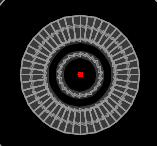
\includegraphics[scale = 0.65]{files/PixeLpART.png}}; 
 \end{tikzpicture}

 \begin{tikzpicture}[overlay, remember picture]
 \node[anchor=center, 
      xshift=3cm, 
      yshift=0cm] 
     at (current page.center)
     {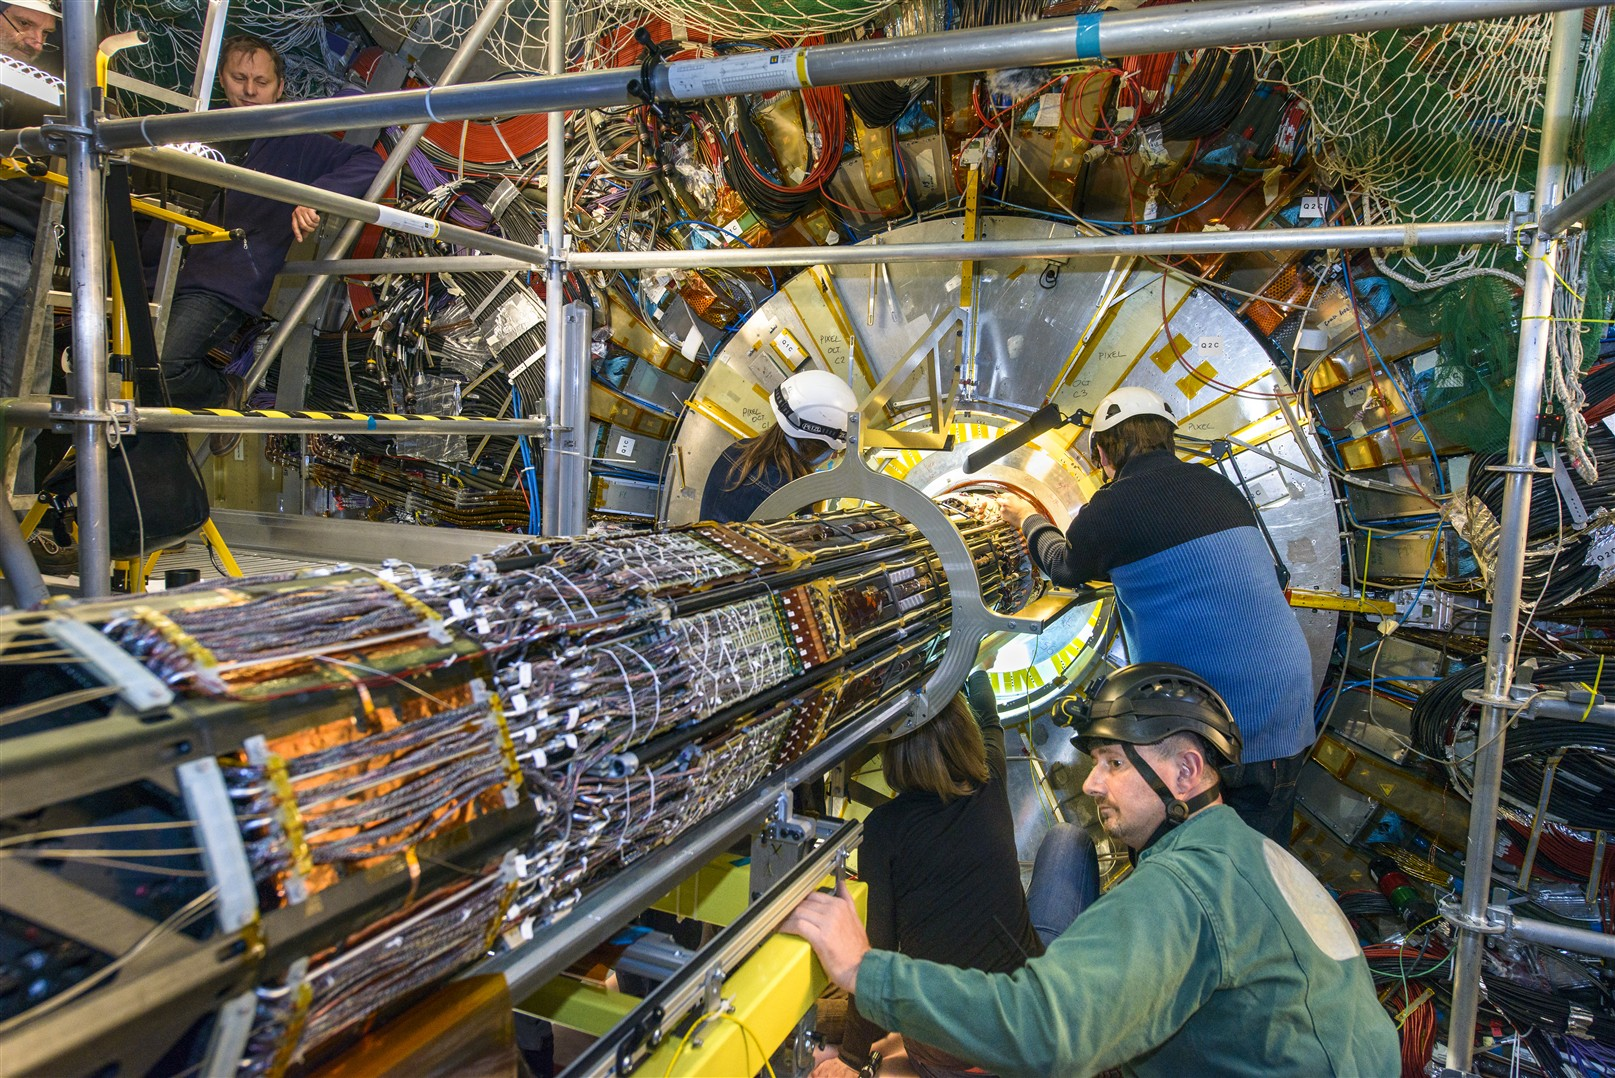
\includegraphics[scale = 0.15]{files/Pix.jpg}}; 
 \end{tikzpicture}

  \begin{tikzpicture}[overlay, remember picture]
 \node[anchor=center, 
      xshift=-0.8cm, 
      yshift=0cm] 
     at (current page.center)
     {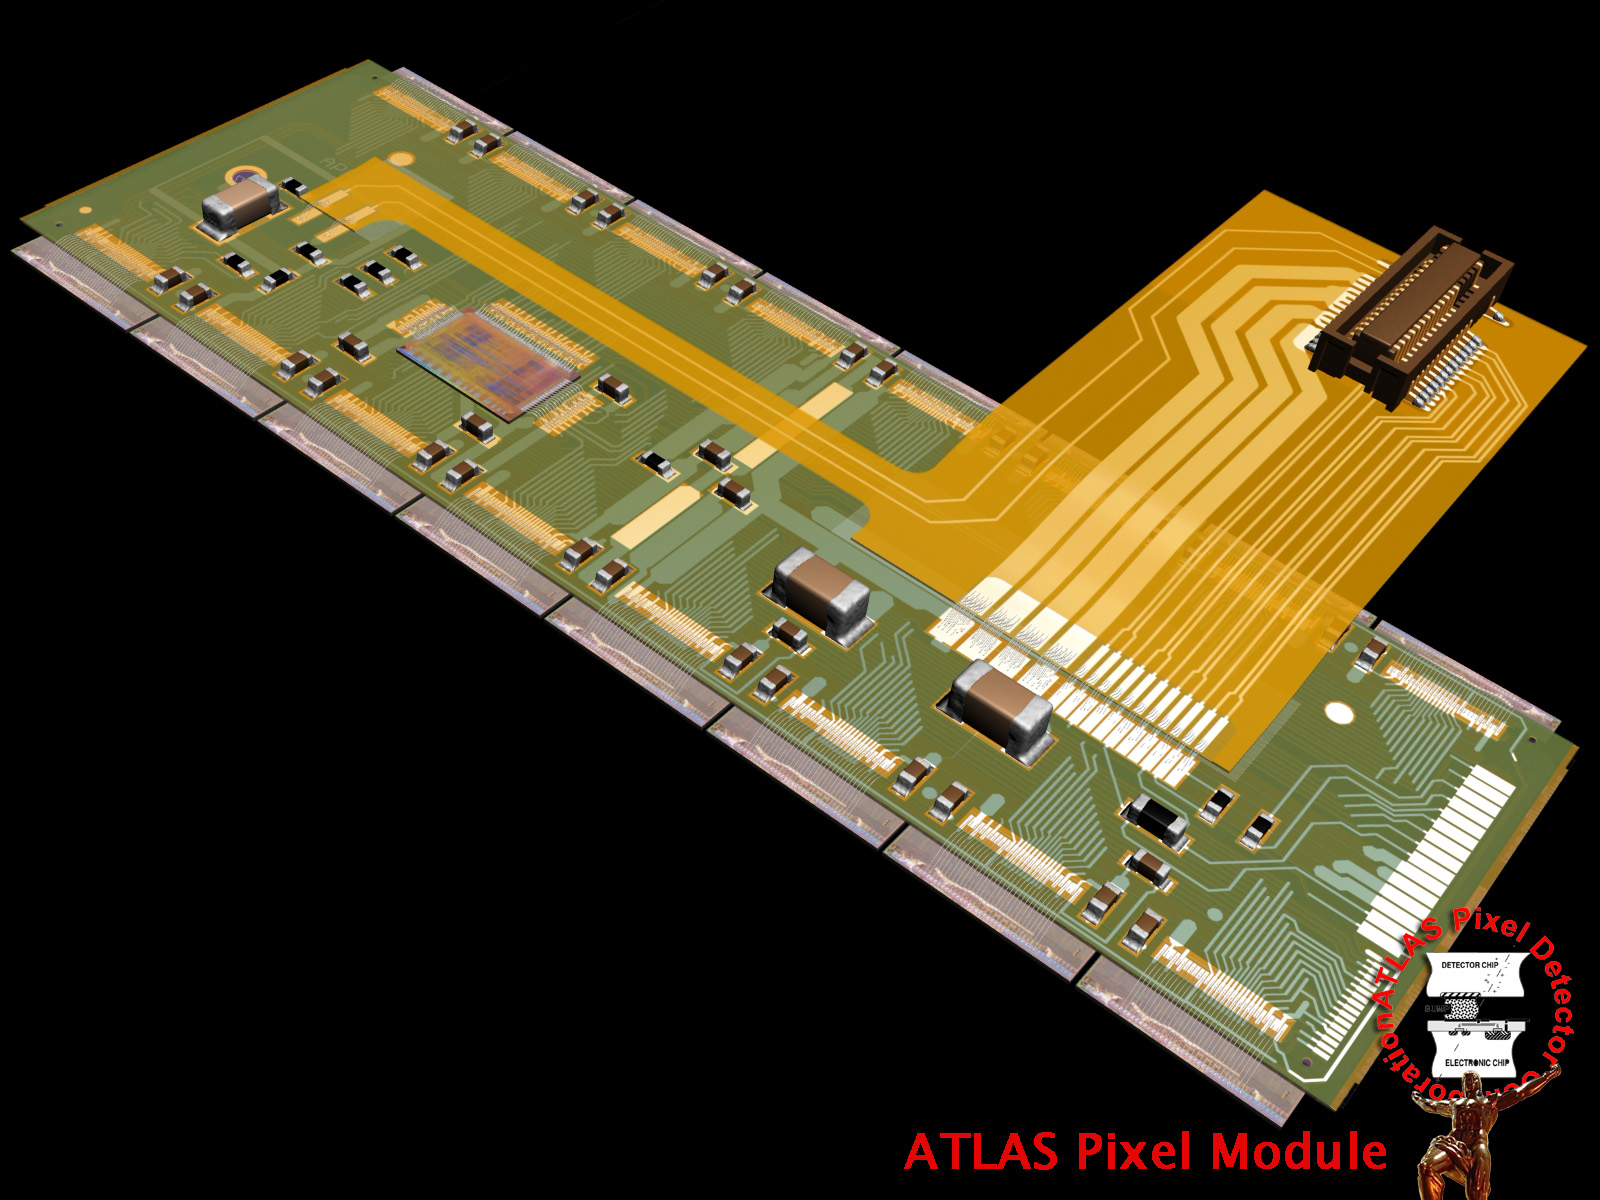
\includegraphics[scale = 0.05]{files/indet-2005-001_10.jpg}}; 
 \end{tikzpicture}

\vspace{2.5cm}
\small
\makebox[1cm]{} \textbf{\textcolor{violet}{Modulele care compun această parte au ca scop principal emiterea unui semnal electric care rezultă ca urmare a ionizărilor multiple induse la traversarea particulelor prin detector- sunt 1744 de module a câte 16 cipuri de cititre fiecare...\href{https://www.youtube.com/watch?v=LGAly8wfhC4}{\textbf{vezi aici logica ingineriei;}}} }
 
\end{frame}


%frame4

\begin{frame}{\textbf{b) \dashuline{Semiconductor Tracker:}}}
 
 \begin{tikzpicture}[overlay, remember picture]
 \node[anchor=center, 
      xshift=-4cm, 
      yshift=-1cm] 
     at (current page.center)
     {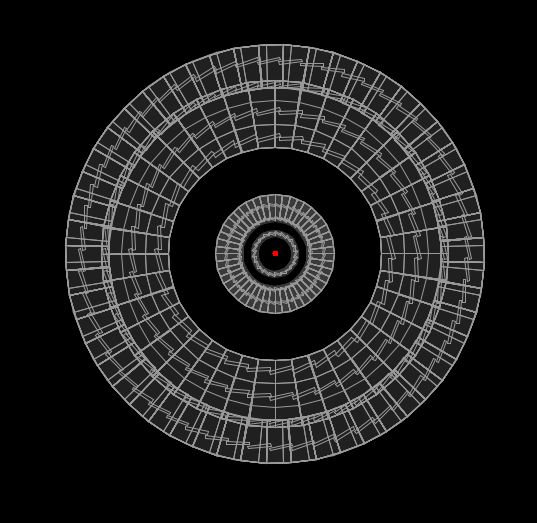
\includegraphics[scale = 0.2]{files/4-Semiconductor Trackes.png}}; 
 \end{tikzpicture}

   \begin{tikzpicture}[overlay, remember picture]
 \node[anchor=center, 
      xshift=-0.8cm, 
      yshift=-1cm] 
     at (current page.center)
     {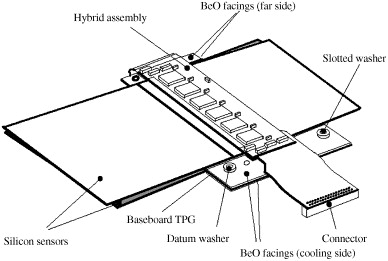
\includegraphics[scale = 1.5]{files/1-s2.0-S016890020601388X-gr2.jpg}}; 
 \end{tikzpicture}

 \begin{tikzpicture}[overlay, remember picture]
 \node[anchor=center, 
      xshift=3cm, 
      yshift=-1cm] 
     at (current page.center)
     {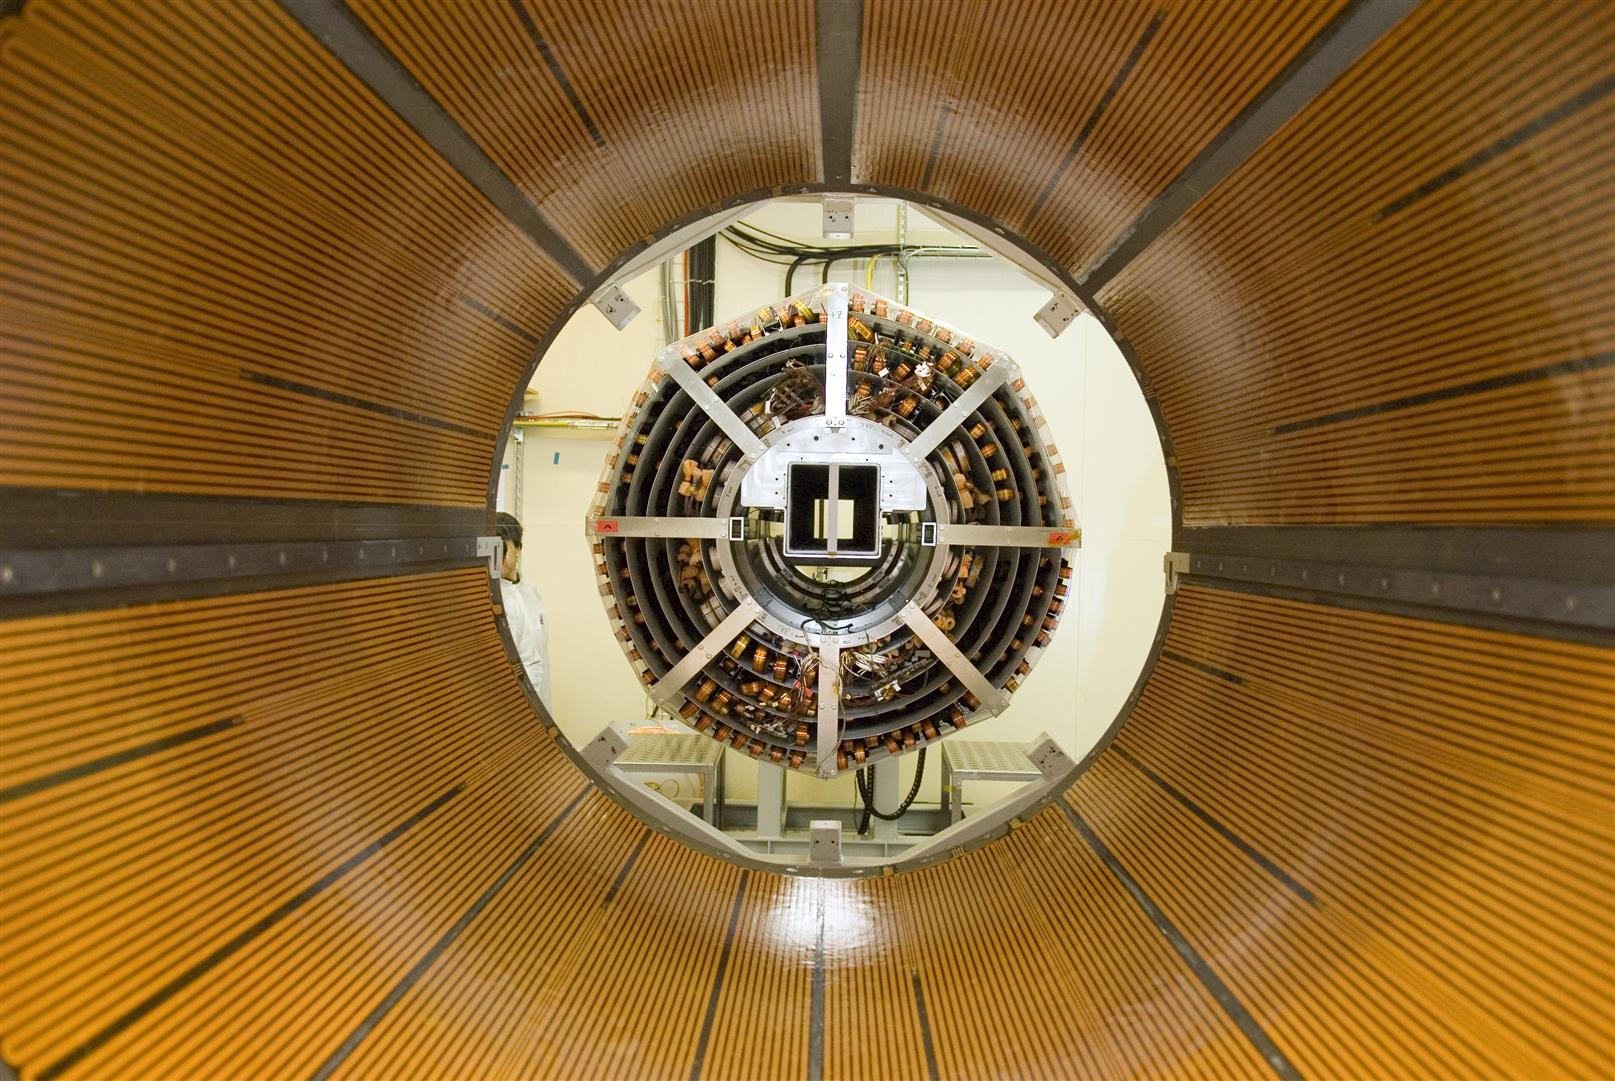
\includegraphics[scale = 0.15]{files/0602009_06-A4-at-144-dpi.jpg}}; 
 \end{tikzpicture}

 \small
 
\vspace{-1.8cm}

\makebox[0.5cm]{}\textbf{ Este utilizat pentru a detecta și reconstrui urmele particulelor încărcate produse în timpul coliziunilor. Se compune din peste 4.000 de module din 6 milioane de "micro-benzi" de senzori de siliciu. \textcolor{red} {Dispunerea sa este optimizată astfel încât fiecare particulă să traverseze cel puțin patru straturi de siliciu.} }

\vspace{4cm}
\begin{itemize}

\item[\ding{34}] \makebox[0.5cm]{}\textbf{ Se compune din 4.088 de module și peste 6 milioane de benzi de citire implantate (6 milioane de canale).}
\end{itemize}

\end{frame}



%frame5 
\begin{frame}{\textbf{b) Alte detalii relevante despre SCT:}}
\small

\begin{itemize}

     \small
    \item[\ding{39}]{\makebox[0.5cm]{} \textit{\textbf{Aproximativ 700 de milioane de coliziuni pot fi detectate de tracker în fiecare secundă.}}}

    \item[\ding{39}]{\makebox[0.5cm]{} \textit{\textbf{Această cantitate de date este mult mai mare decât ceea ce poate fi procesat, stocat sau analizat de experiment.}}}
  
    \item[\ding{39}]{\makebox[0.5cm]{} \textit{\textbf{Datele de la tracker sunt, prin urmare, foarte importante pentru a stabili care coliziuni sunt interesante și merită păstrate și care pot fi aruncate ca evenimente "de fundal" neinteresante.}}}
  
    \item[\ding{39}]{\makebox[0.5cm]{} \textit{\textbf{Ca urmare, mai puțin de una dintr-un milion de coliziuni detectate în tracker sunt înregistrate vreodată pe disc pentru o analiză ulterioară.}}}

    \item[\ding{39}]{\makebox[0.5cm]{} \textit{\textbf{Împreună cu detectorul de pixeli din centrul ATLAS, acest tracker operează sincron pentru a măsura cu precizie căile(pathurile) particulelor care rezultă din coliziunile extrem de energetice.}}}
    
\end{itemize}

\end{frame}



%frame6 -> in continuare

\begin{frame}{\textbf{c)\dashuline{ Transition Radiation Tracker- inelul albastru:}}}

\vspace{-0.5cm}
\small
\makebox[0.5cm]{} \textbf{TRT este format din 300.000 de tuburi cu pereți subțiri (sau paie). 
Fiecare tub are doar 4 mm în diametru, cu un fir de tungsten placat cu un strat de aur de 30 micrometrii în centru.}
 
 \begin{tikzpicture}[overlay, remember picture]
 \node[anchor=center, 
      xshift=-3.5cm, 
      yshift=0cm] 
     at (current page.center)
     {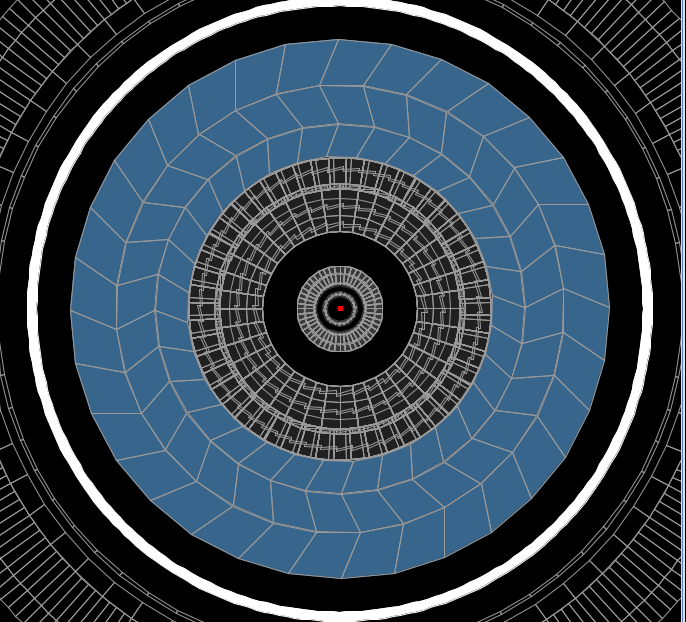
\includegraphics[scale = 0.21]{files/5-TRT- transition radiation tracker.png}}; 
 \end{tikzpicture}


 \begin{tikzpicture}[overlay, remember picture]
 \node[anchor=center, 
      xshift=2.5cm, 
      yshift=0cm] 
     at (current page.center)
     {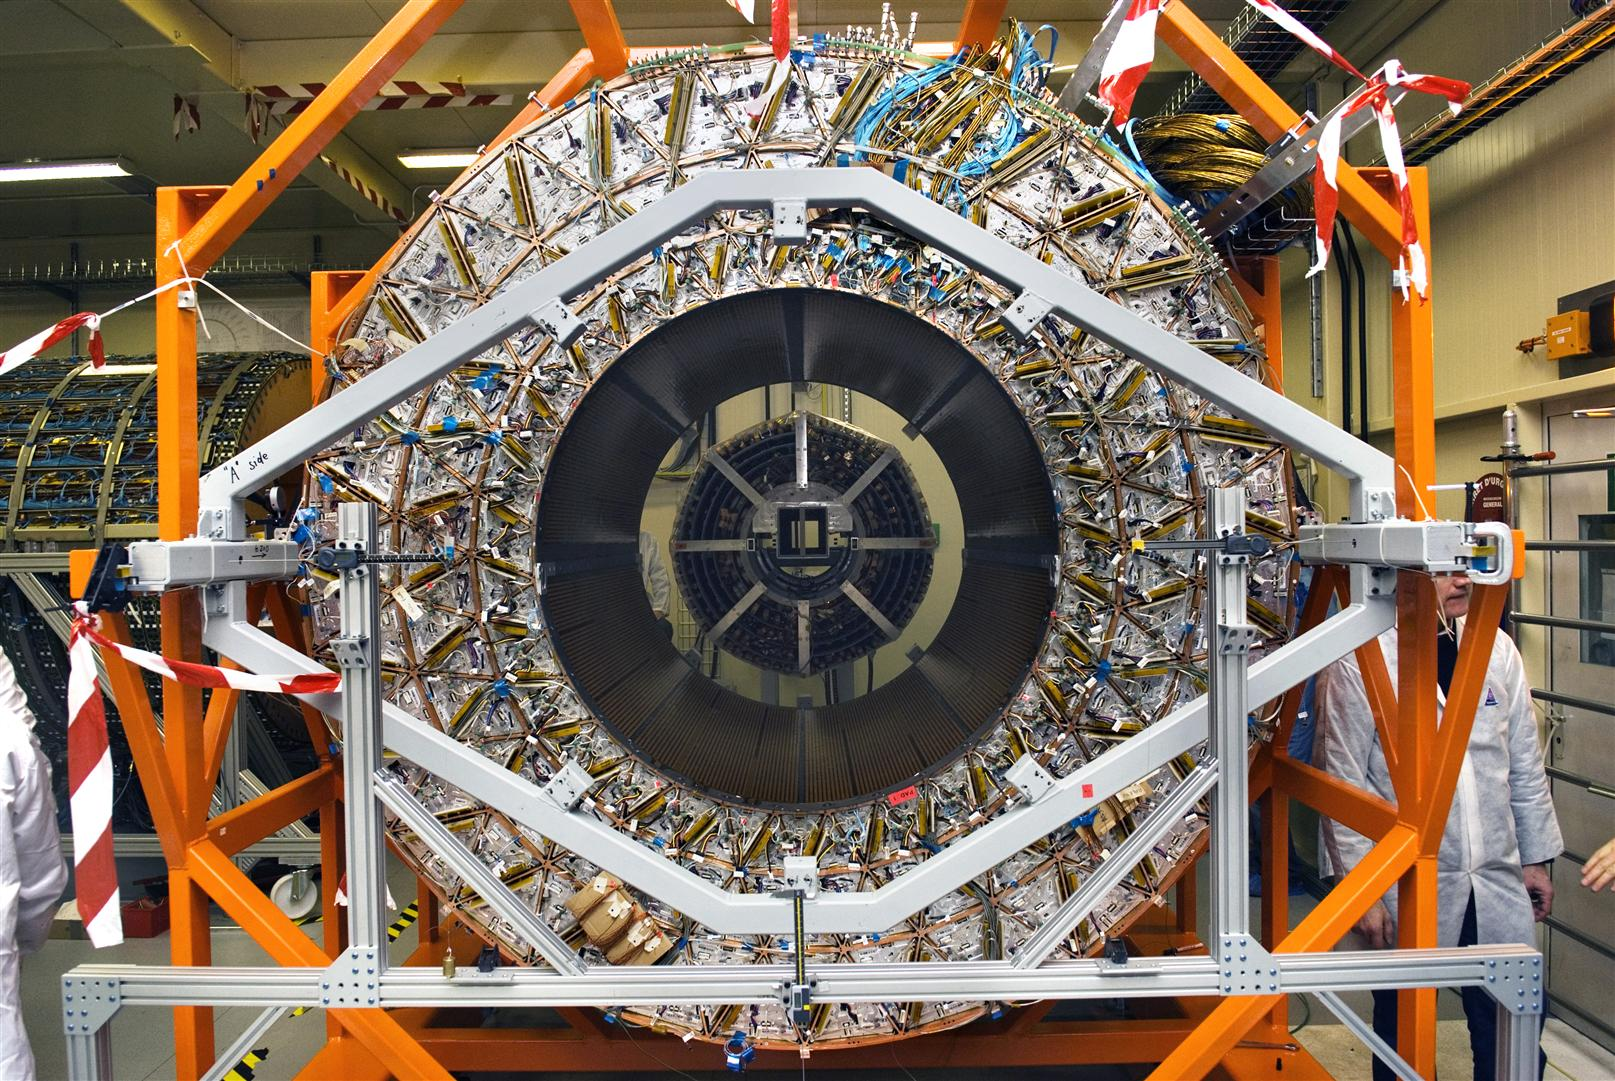
\includegraphics[scale = 0.19]{files/TRT.jpg}}; 
 \end{tikzpicture}

\vspace{3.5cm}
 \makebox[0.5cm]{} \textbf{ \textit{\textcolor{magenta}{Pe măsură ce particulele încărcate trec prin paie, ele ionizează gazul pentru a crea un semnal electric detectabil. Ulterior acest semnal analog este convertit într-unul digital. }}}

\end{frame}


%frame7

\begin{frame}{\href{https://www.youtube.com/watch?v=gljjW2Pqz5g&t=410s}{\textbf{c) mecanismul TRT:}}}

\vspace{-0.5cm}

\small

\begin{itemize}

\small 
\item[\ding{66}]\makebox[0.5cm]{} \textcolor{blue}{\textbf{\textit{
Semnalul electric rezultat prin ionizarea gazului din tuburi este folosit pentru a reconstrui urmele particulelor și, datorită așa-numitei radiații de tranziție, oferă informații despre tipul de particule cu sarcină care au trecut prin detector(electroni sau pioni).}}}

\end{itemize}

 \begin{tikzpicture}[overlay, remember picture]
 \node[anchor=center, 
      xshift=-2cm, 
      yshift=0cm] 
     at (current page.center)
     {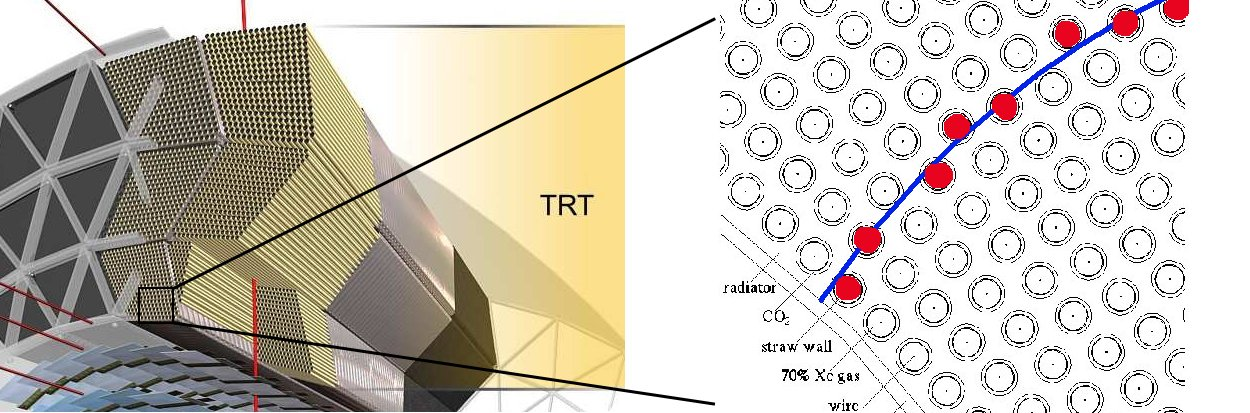
\includegraphics[scale = 0.4]{files/ATLAS_TRT_Principle_image.jpg}}; 
 \end{tikzpicture}


 \begin{tikzpicture}[overlay, remember picture]
 \node[anchor=center, 
      xshift=4cm, 
      yshift=0cm] 
     at (current page.center)
     {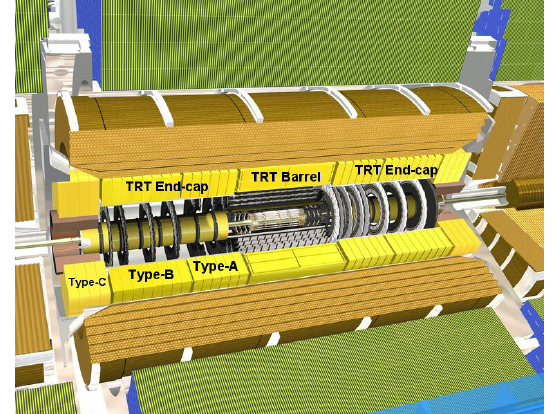
\includegraphics[scale = 0.23]{files/ATLAS-Transition-Radiation-Tracker.png}}; 
 \end{tikzpicture}


 \vspace{3cm}

\small

\begin{itemize}

\small 
\item[\ding{66}]\makebox[0.5cm]{} \textcolor{gray}{\textbf{\textit{Toate cele 3 componente(a,b și c) ale detectorului interior sunt plasate într-un câmp magnetic de cca. 2T, generat de un solenoid central(inelul alb).}}}

\end{itemize}

\end{frame}



%frame7 -> in continuare




%frame8 -> in continuare LAr
\begin{frame}{\dotuline{d) \href{https://www.youtube.com/watch?v=gljjW2Pqz5g}{ Calorimetrul cu Argon Lichid(LAr)- inelul verde;}}}

\vspace{-3cm}


\begin{itemize}

\small
\item[\ding{88}]\makebox[0.5cm]{} \textbf{\textcolor{red}{Măsoară energia electronilor, fotonilor și hadronilor cu sarcină nenulă.} Dispune de straturi de metal (fie wolfram, cupru sau plumb) care absorb particulele captate, transformându-le într-un flux de particule noi, cu energie mai mică. \textit{Aceste particule ionizează argonul lichid cuprins între straturi, producând un curent electric măsurabil.}}

\end{itemize}

 \begin{tikzpicture}[overlay, remember picture]
 \node[anchor=center, 
      xshift=-2.4cm, 
      yshift=-1.9cm] 
     at (current page.center)
     {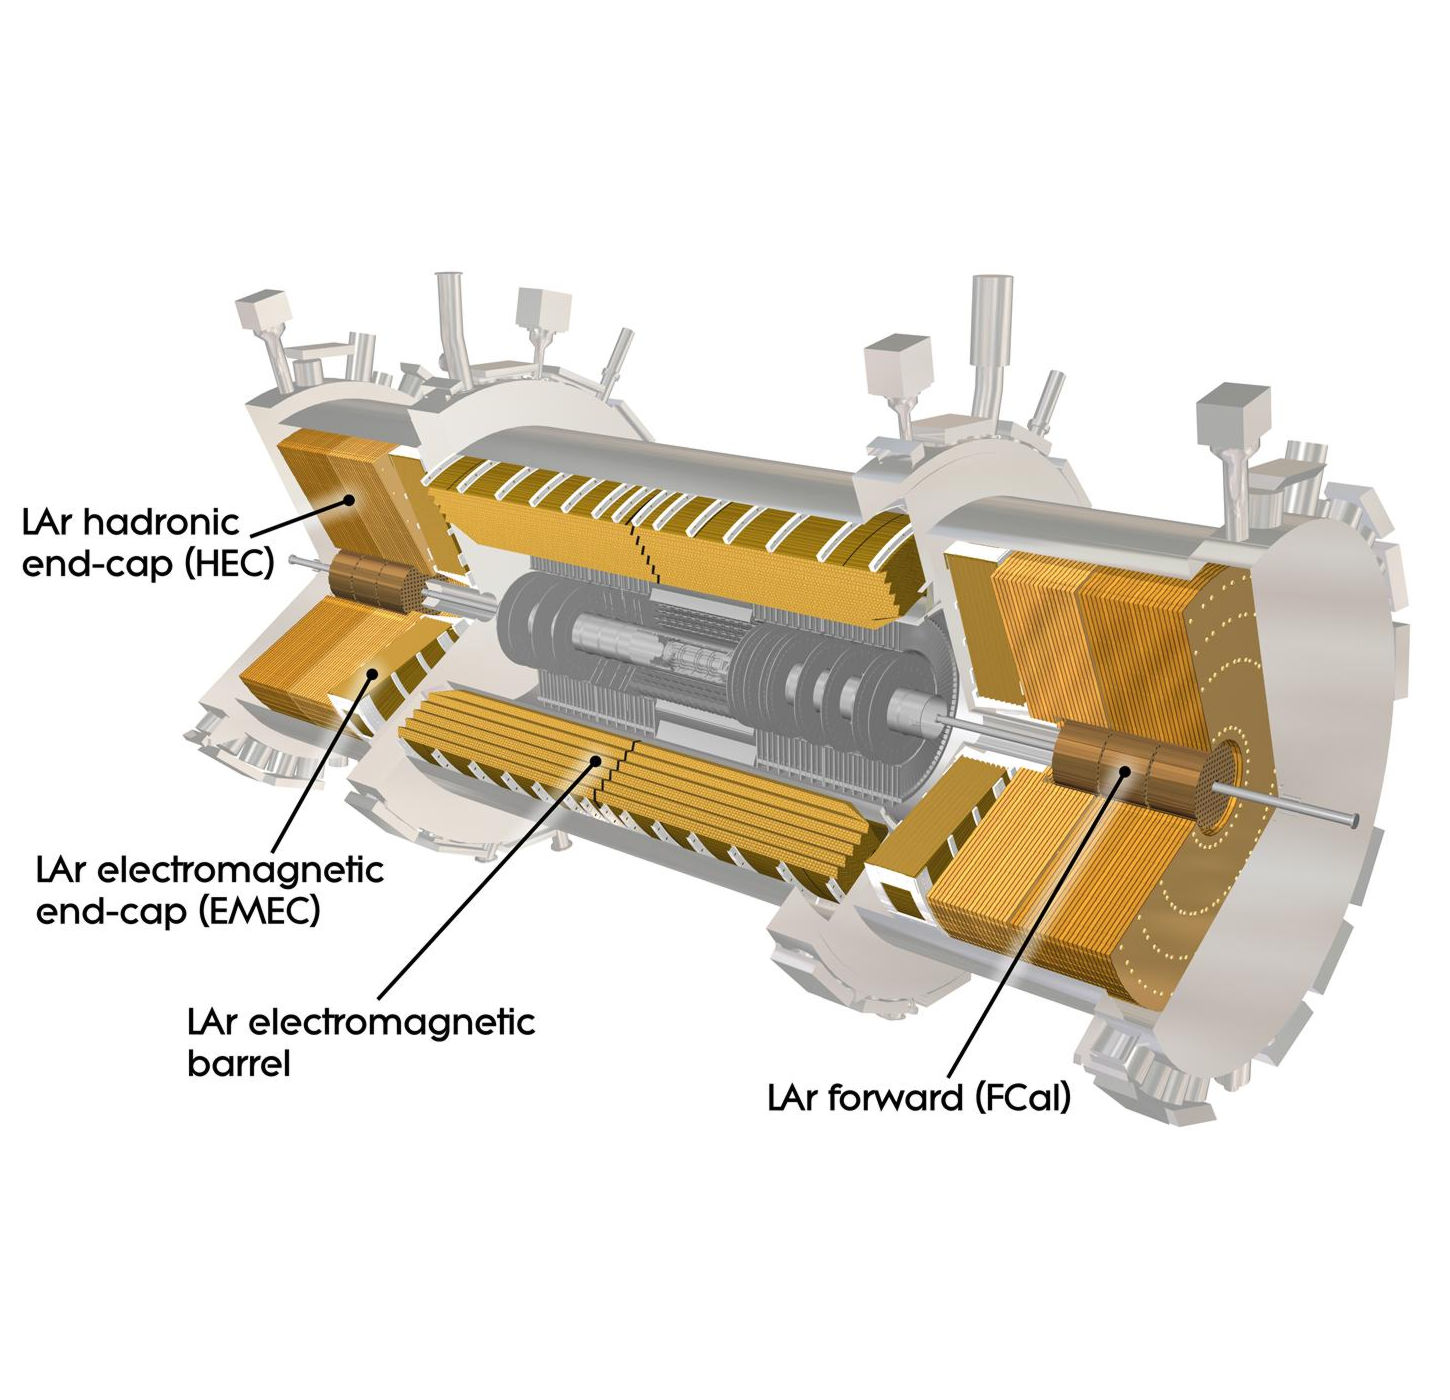
\includegraphics[scale = 0.12]{files/LAr_Calorimeter.jpg}}; 
 \end{tikzpicture}

  \begin{tikzpicture}[overlay, remember picture]
 \node[anchor=center, 
      xshift=3cm, 
      yshift=-1cm] 
     at (current page.center)
     {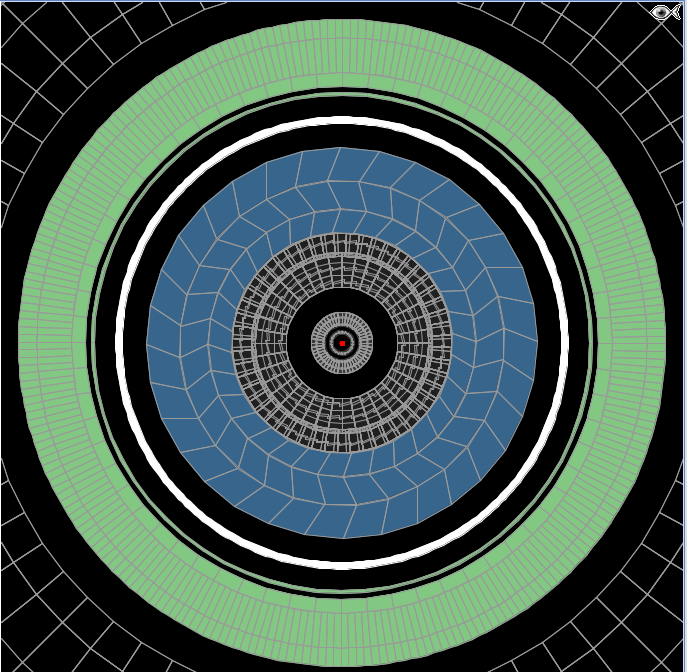
\includegraphics[scale = 0.21]{files/7-LAr-CalorimetrulELM.png}}; 
 \end{tikzpicture}

\end{frame}

%frame9 -> in continuare LAr
\begin{frame}{\textbf{LAr- detalii de substrat}}

\vspace{-0.5cm}

\begin{itemize}
 \small
    \item[1)] \makebox[0.5cm]{}  \textit{\textbf{Regiunea centrală a calorimetrului electromagnetic este special concepută pentru a identifica electronii și fotonii.}} \\

    ........................................................................................................
    
    \item[2)] \makebox[0.5cm]{}  \textit{\textbf{Are o structură de acordeon caracteristică( model de fagure), cu straturi de Pb și oțel între care se află argon lichefiat.}}\\

    ........................................................................................................

    \item[3)] \makebox[0.5cm]{}  \textit{\textbf{Pentru a păstra argonul în formă lichidă, calorimetrul este menținut la -184°C. Cilindrii de cabluri special proiectați, sigilați în vid, receptează și aduc semnalele electronice de la argonul lichid rece în zona caldă unde sunt și electronicele de citire.}}\\

    ........................................................................................................

    \item[4)] \makebox[0.5cm]{}  \textit{\textbf{Particula energică cu sarcină nenulă pătrunde în straturile structurii și ionizează atomii de argon, lăsând în urmă sarcini libere negative care sunt mai apoi captate de electrodul din Cu al unei grile.}}\\

    ........................................................................................................

    \item[5)] \makebox[0.5cm]{}  \textit{\textbf{Prin combinarea tuturor curenților detectați astfel, fizicienii pot determina energia particulei originale care a lovit detectorul.}}
    
\end{itemize}

\end{frame}


%frame10- Hadronic Calorimeter TILE

\begin{frame}{d) \dotuline{\href{https://www.youtube.com/watch?v=gljjW2Pqz5g}{Calorimetrul Hadronic(Tile)- inelul roșu;}}}

\vspace{-2.5cm}

\begin{itemize}

\small

\item [\ding{88}]\makebox[0.5cm]{} \textit{\textbf{\textcolor{gray}{Măsoară energia particulelor hadronice, care nu depun toată energia lor în calorimetrul LAr.} \textcolor{cyan}{Este realizat din straturi de oțel și plăci scintilante iar pe măsură ce particulele lovesc straturile de oțel, ele generează o ploaie de particule noi. }}}

\end{itemize}

 \begin{tikzpicture}[overlay, remember picture]
 \node[anchor=center, 
      xshift=-2.4cm, 
      yshift=-1cm] 
     at (current page.center)
     {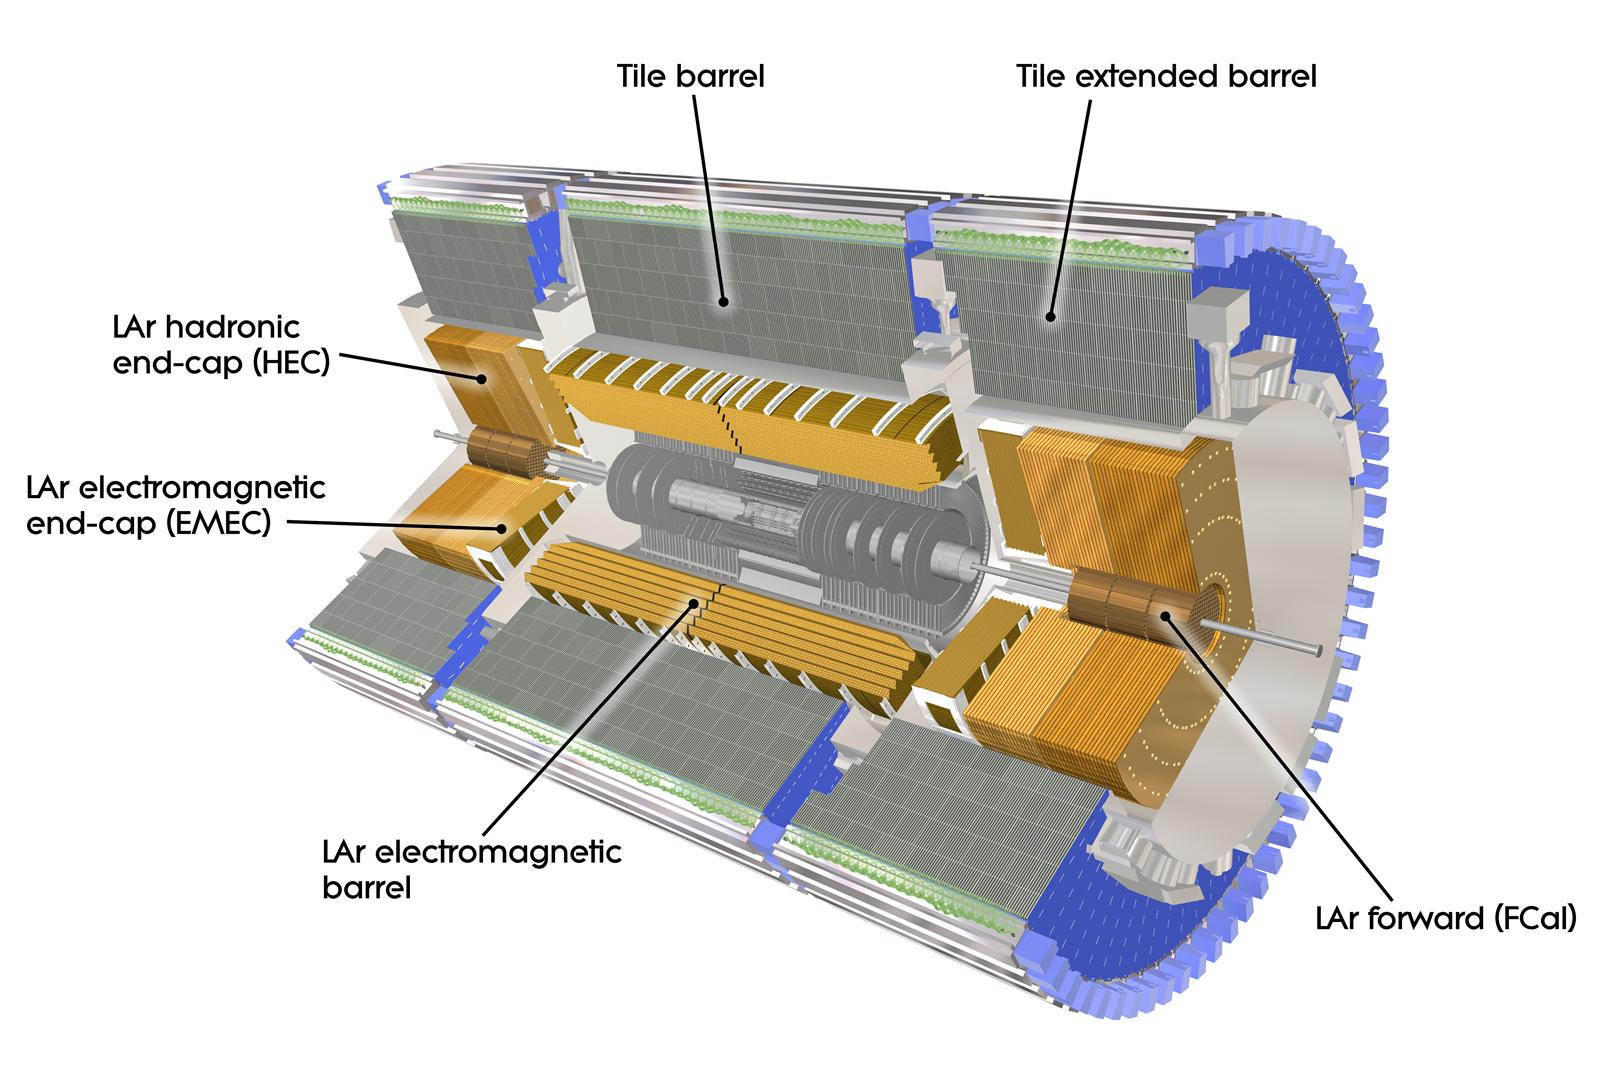
\includegraphics[scale = 0.23]{files/file.jpg}}; 
 \end{tikzpicture}

  \begin{tikzpicture}[overlay, remember picture]
 \node[anchor=center, 
      xshift=3cm, 
      yshift=-1cm] 
     at (current page.center)
     {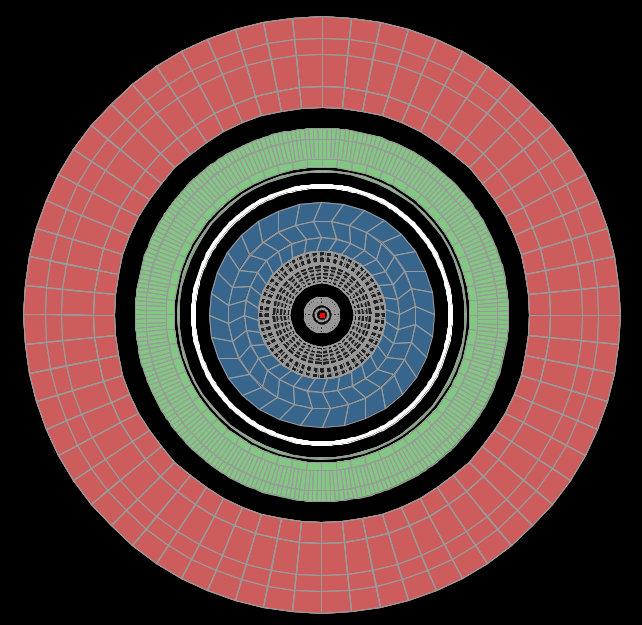
\includegraphics[scale = 0.22]{files/8-CalorimetrulHadronic.png}}; 
 \end{tikzpicture}

\end{frame}


%frame11- Hadronic Calorimeter TILE - detalii de substrat;

\begin{frame}{\href{https://atlas.cern/Discover/Detector/Calorimeter}{Calorimetrul Hadronic- pentru mai multe detalii:}}

\begin{enumerate}

 \small
    \item[1)] \makebox[0.5cm]{}  \textit{\textbf{Calorimetrul hadronic este un "array" de plăci din oțel și scintilatoare(~420.000), dispuse în paralel.}} \\

    ---------------------------------------------------------------------------------------
    
    \item[2)] \makebox[0.5cm]{}  \textit{\textbf{Pe măsură ce hadronul pătrunde în straturile acestui calorimetru, inițiază reacții nucleare cu atomii din plăci, reacții care formează dușuri de particule secundare printre care și radiații ionizante.}}\\

    ---------------------------------------------------------------------------------------

    \item[3)] \makebox[0.5cm]{}  \textit{\textbf{Radiațiile de înaltă energie pătrund mai apoi în scintilatoare și produc emisia de fotoni.}}\\

    ---------------------------------------------------------------------------------------

    \item[4)] \makebox[0.5cm]{}  \textit{\textbf{Fotonii sunt captați prin fibre și convertiți în semnale analogice(curent electric)}}\\

    ---------------------------------------------------------------------------------------

    \item[5)] \makebox[0.5cm]{}  \textit{\textbf{Indirect, pe baza energiei/intensității radiației luminoase se poate deduce cât este energia medie a hadronilor(mezoni, protoni) de input}}
    
\end{enumerate}
\end{frame}


%Spectrometrul Muonic

\begin{frame}{\dotuline{d) \href{https://www.youtube.com/watch?v=gljjW2Pqz5g}{{Spectrometrul Muonic - partea exterioară;}}}}

\vspace{-3cm}


\begin{itemize}


\item[\ding{76}]\makebox[0.5cm]{} \textbf{\textcolor{red}{Spectrometrul muonic este alcătuit dintr-o serie de câteva mii de camere și este stratul cel mai exterior al detectorului ATLAS. Identifică și măsoară impulsul muonilor produși din coliziune..}}

\end{itemize}

%imag1
 \begin{tikzpicture}[overlay, remember picture]
 \node[anchor=center, 
      xshift=-2.4cm, 
      yshift=-1cm] 
     at (current page.center)
     {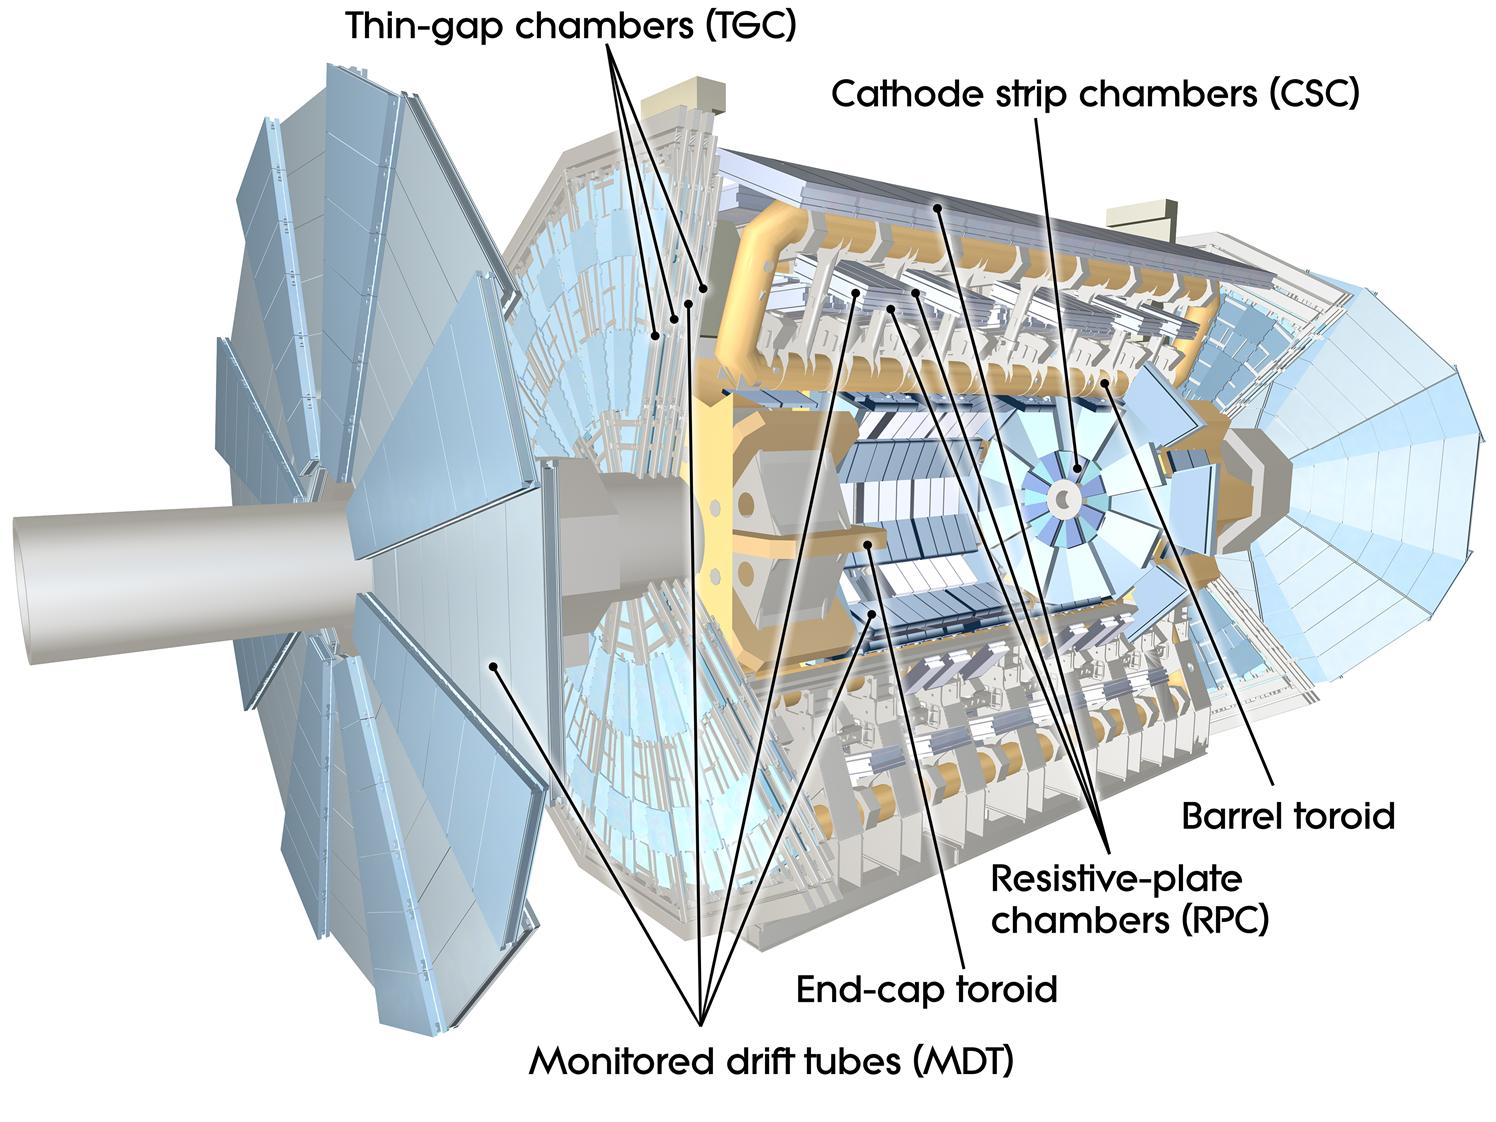
\includegraphics[scale = 0.2]{files/MuonCh,bers.jpg}}; 
 \end{tikzpicture}

%imag2
  \begin{tikzpicture}[overlay, remember picture]
 \node[anchor=center, 
      xshift=3cm, 
      yshift=-1cm] 
     at (current page.center)
     {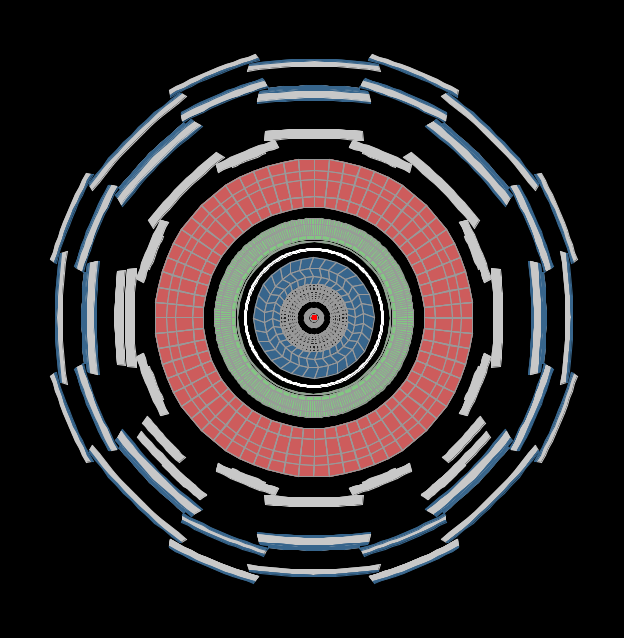
\includegraphics[scale = 0.25]{files/10-MDT.png}}; 
 \end{tikzpicture}

\end{frame}


%ultima parte din ansamblu- Muon chambers:
\begin{frame}{\textit{\href{https://atlas.cern/Discover/Detector/Muon-Spectrometer}{Spectrometrul Muonic - aspecte relevante:}}}

\vspace{-1cm}

\begin{enumerate}
 \small
    \item[a)] \makebox[0.5cm]{}  \textit{\textbf{ Elementele de detectare (camerele muonice) sunt realizate din mii de tuburi metalice echipate cu un fir central și umplute cu gaz.}} \\

    ---------------------------------------------------------------------------------------
    
    \item[b)] \makebox[0.5cm]{}  \textit{\textbf{Pe măsură ce un muon trece prin aceste tuburi, el lasă o urmă o dâră de ioni și electroni încărcați electric care se deplasează în lateral și către centrul tubului.}}\\

    ---------------------------------------------------------------------------------------

    \item[c)] \makebox[0.5cm]{}  \textit{\textbf{ Măsurând timpul necesar pentru ca aceste sarcini să se deplaseze de la punctul de plecare către firul central(într-o mișcare de drift) sau spre marginile tubului, este posibil să se determine poziția aproximativă a muonului pe măsură ce trece prin el.}}\\

    ---------------------------------------------------------------------------------------

    \item[d)] \makebox[0.5cm]{}  \textit{\textbf{ Sunt cca. 4000 de camere muonice individuale! Scopul este de a detecta prezența acestor particule energice.}}\\

\end{enumerate}
\end{frame}


%sistemul de magneti
\begin{frame}{e) \dotuline{\href{https://atlas.cern/Discover/Detector/Magnet-System}{Solenoidul Central;}}}

\vspace{-2.5cm}

\begin{itemize}

\small

\item [\ding{74}]\makebox[0.5cm]{} \textit{\textbf{\textcolor{gray}{Solenoidul central ATLAS} înconjoară detectorul interior și generează un câmp magnetic de 2 Tesla, cu o grosime de doar 4.5 cm. Este realizat prin încorporarea a peste 9 km de fire superconductoare niobiu-titan în benzi de aluminiu întărite, pure, minimizând astfel posibilele interacțiuni dintre magnet și particulele studiate.}}

\end{itemize}

%imag1
 \begin{tikzpicture}[overlay, remember picture]
 \node[anchor=center, 
      xshift=-3cm, 
      yshift=-1.2cm] 
     at (current page.center)
     {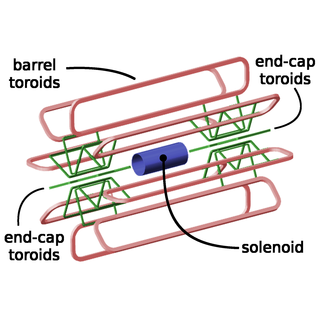
\includegraphics[scale = 0.5]{files/f5000d023ce9c928da8c5ee76949e61b.png}}; 
 \end{tikzpicture}

%imag2
  \begin{tikzpicture}[overlay, remember picture]
 \node[anchor=center, 
      xshift=3cm, 
      yshift=-1.2cm] 
     at (current page.center)
     {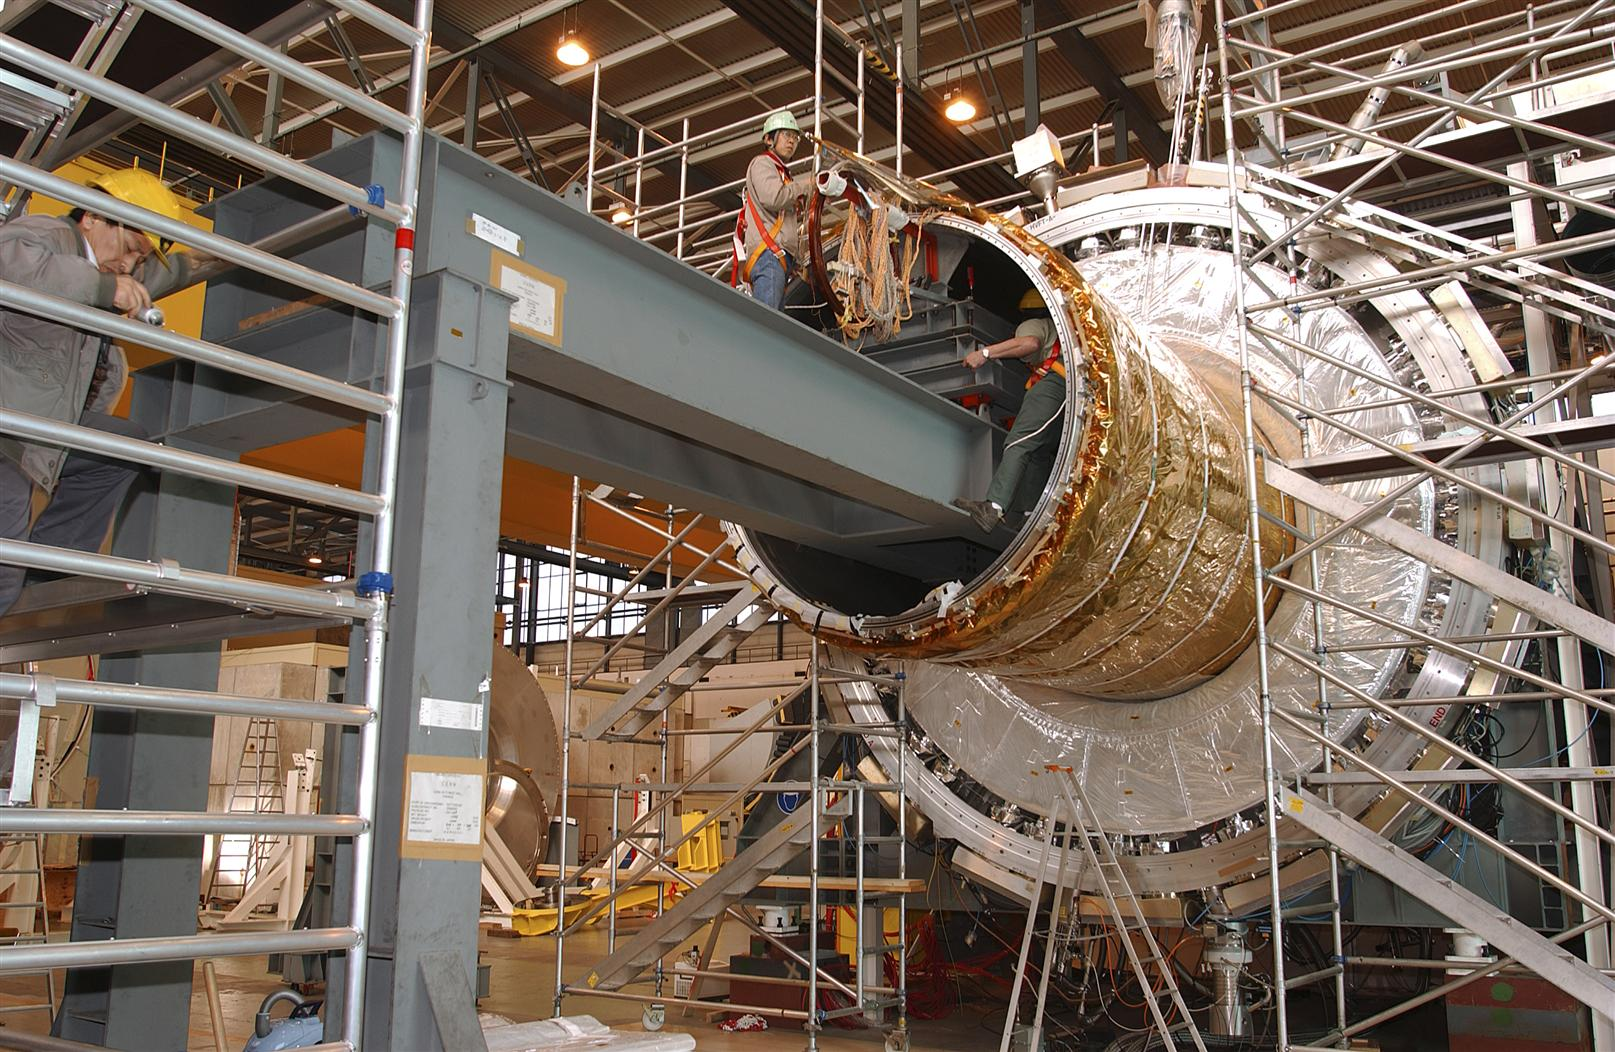
\includegraphics[scale = 0.2]{files/Mag.jpg}}; 
 \end{tikzpicture}

\end{frame}

%magnetii toroidali
\begin{frame}{f) \dotuline{\href{https://atlas.cern/Discover/Detector/Magnet-System}{Magneții toroidali:}}}

\vspace{-2.5cm}

\begin{itemize}

\small

\item [\ding{74}]\makebox[0.5cm]{} \textit{\textbf{\textcolor{red}{Magneții toroidali} ATLAS folosesc o serie de opt bobine pentru a furniza un câmp magnetic de până la 3.5 Tesla, utilizat pentru a măsura impulsul muonilor. Există trei magneți toroidali în ATLAS: doi la sfârșitul experimentului și un toroid masiv care înconjoară centrul experimentului.}}

\end{itemize}

%imag1
 \begin{tikzpicture}[overlay, remember picture]
 \node[anchor=center, 
      xshift=-3cm, 
      yshift=-1.2cm] 
     at (current page.center)
     {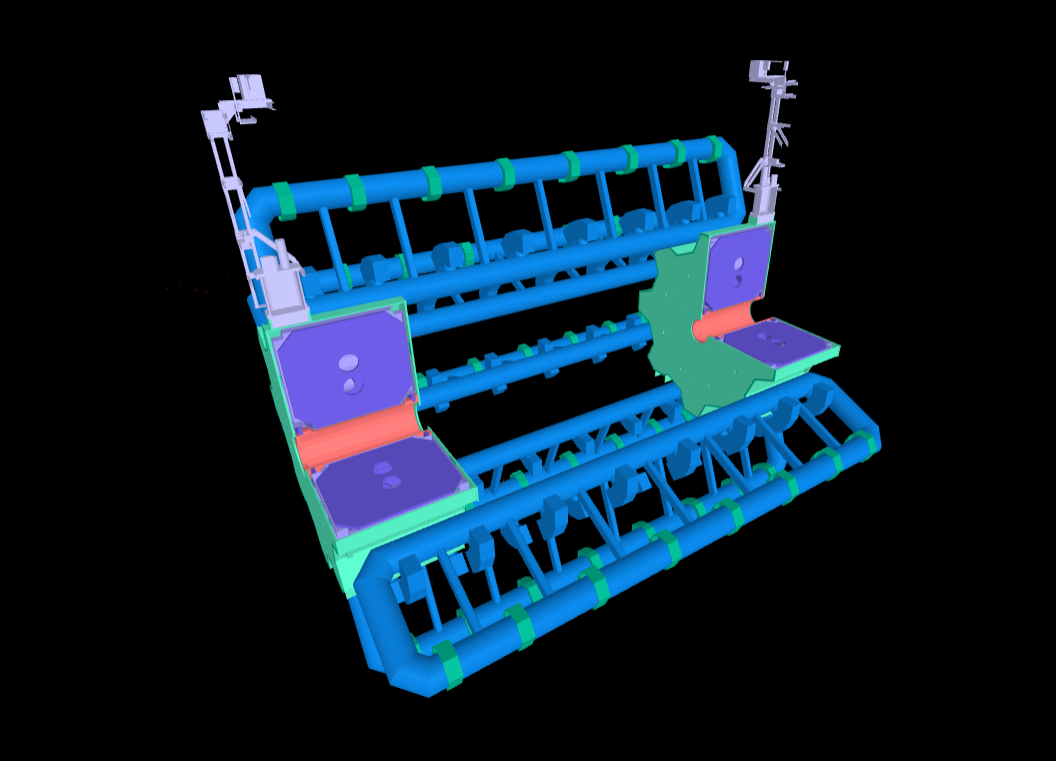
\includegraphics[scale = 0.25]{files/af.png}}; 
 \end{tikzpicture}

%imag2
  \begin{tikzpicture}[overlay, remember picture]
 \node[anchor=center, 
      xshift=3cm, 
      yshift=-1.2cm] 
     at (current page.center)
     {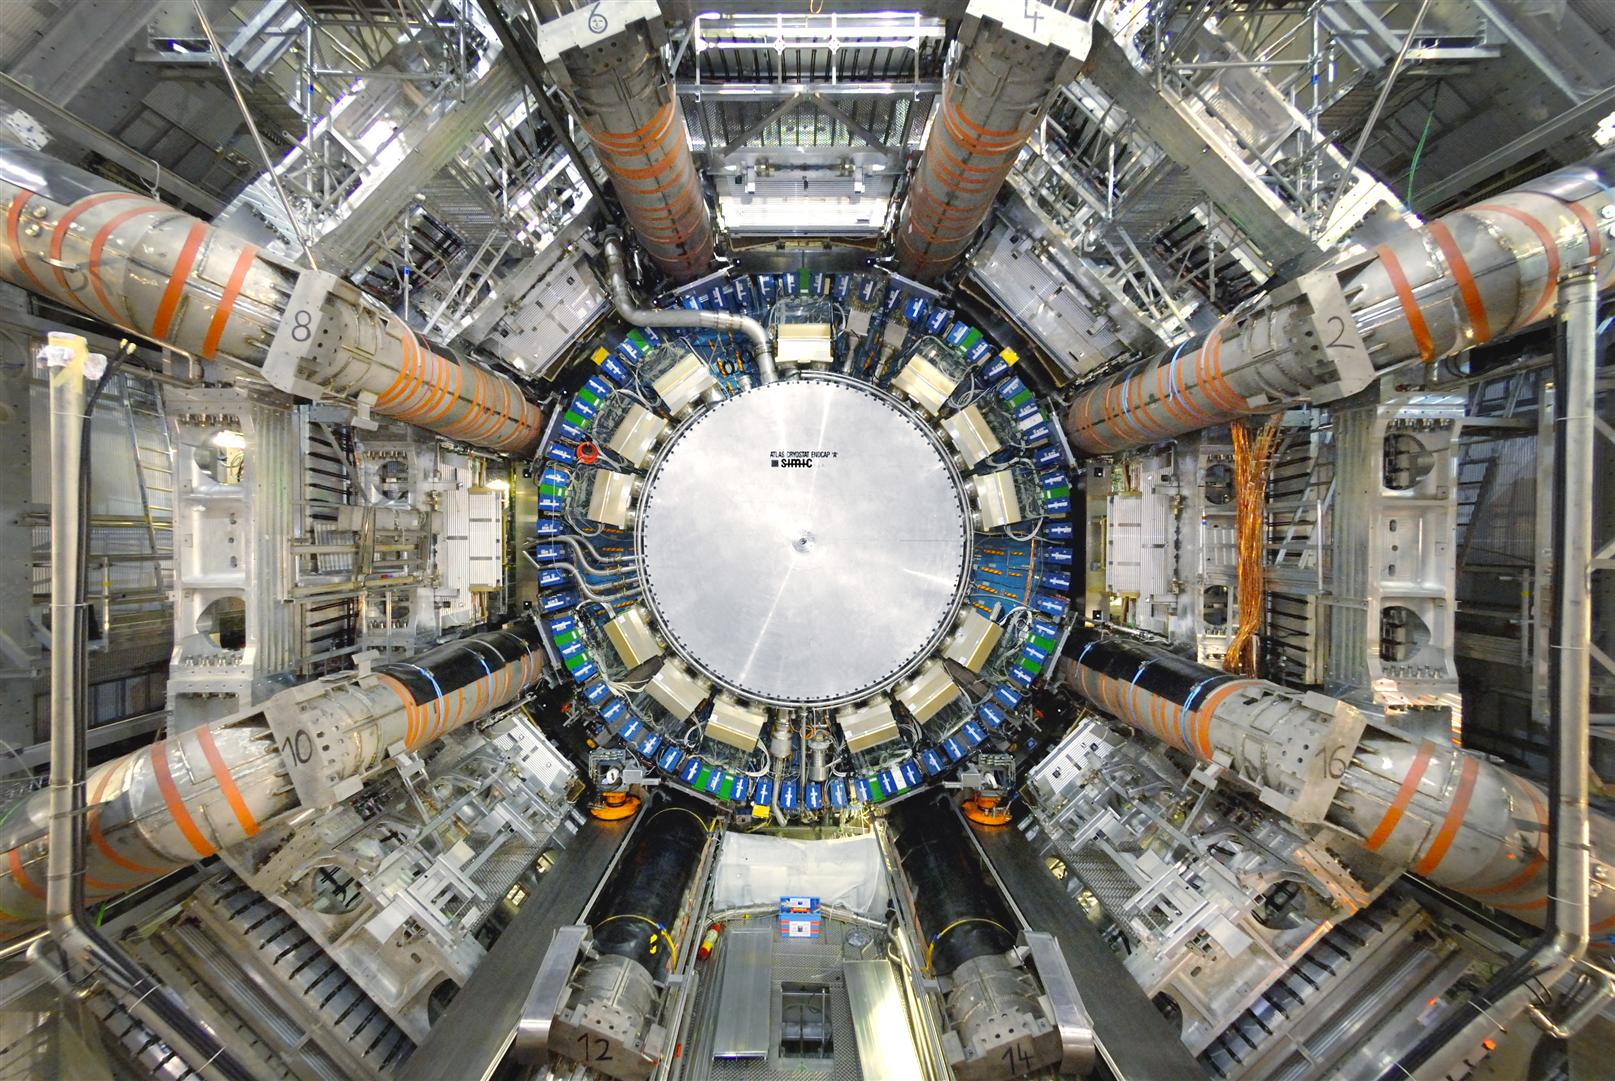
\includegraphics[scale = 0.2]{files/Toroid.jpg}}; 
 \end{tikzpicture}

\end{frame}


%frame tracks-uri date

\begin{frame}{\dotuline{Cum arată amprentele ilustrate ale particulelor detectabile?}}
\vspace{-3.5cm}
\small

\begin{itemize}
\item [\ding{55}] \makebox[0.5cm]{} \textit{\textbf{ Fiecare particulă stabilă sau cu un timp semnificativ de viață induce variații proprii în straturile detectoare; particulele neutre electric și foarte penetrante sunt cel mai dificil de reperat (cum ar fi neutrinul care este cu totul invizibil pentru detectori);}}
\end{itemize}


 \begin{tikzpicture}[overlay, remember picture]
 \node[anchor=center, 
      xshift=-2.4cm, 
      yshift=-1.3cm] 
     at (current page.center)
     {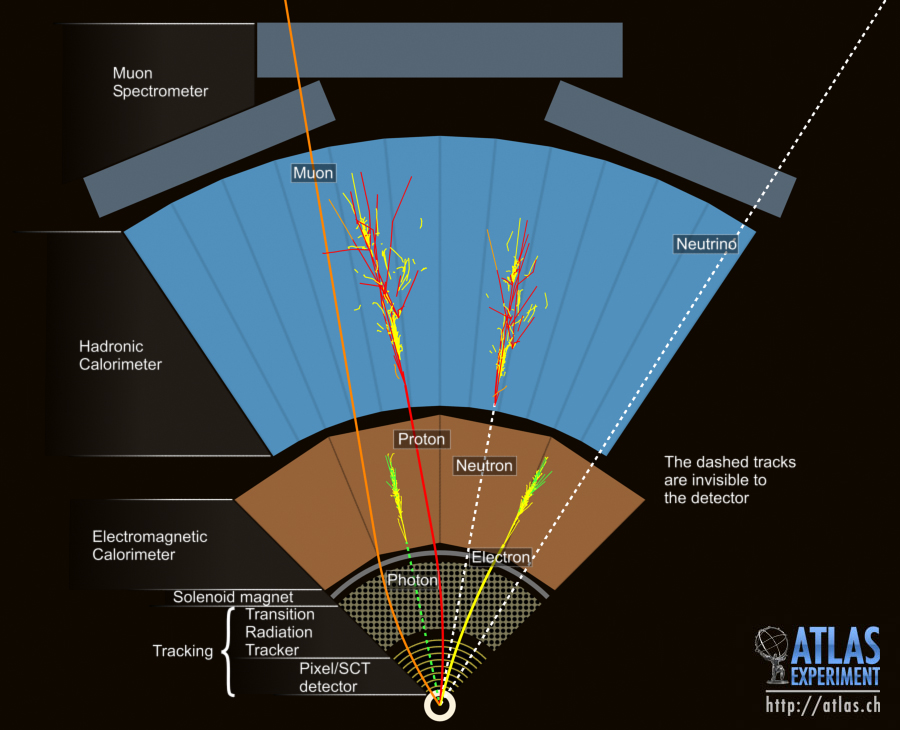
\includegraphics[scale = 0.2]{files/lhc_atlas_dection.jpg}}; 
 \end{tikzpicture}

  \begin{tikzpicture}[overlay, remember picture]
 \node[anchor=center, 
      xshift=3.3cm, 
      yshift=-1cm] 
     at (current page.center)
     {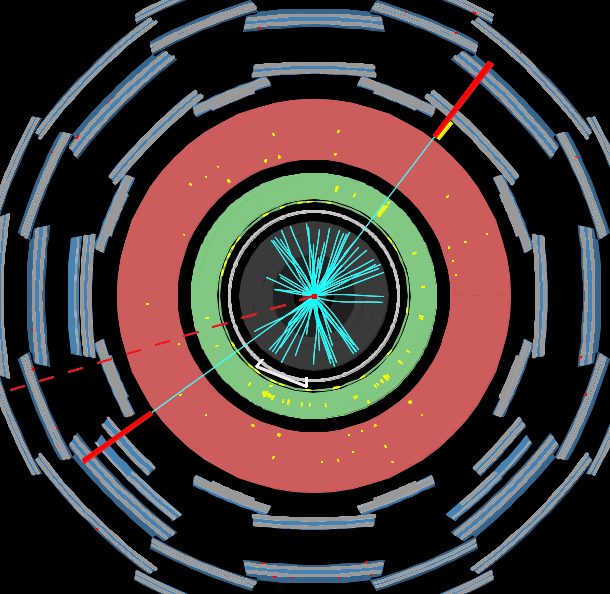
\includegraphics[scale = 0.27]{files/trajectories.png}}; 
 \end{tikzpicture}


\end{frame}


%frame tracks-uri date

%muons tracks
\begin{frame}{\dashuline{}{\textbf{1) Semnătura muonilor.}}}


 \begin{tikzpicture}[overlay, remember picture]
 \node[anchor=center, 
      xshift=0cm, 
      yshift=-0.3cm] 
     at (current page.center)
     {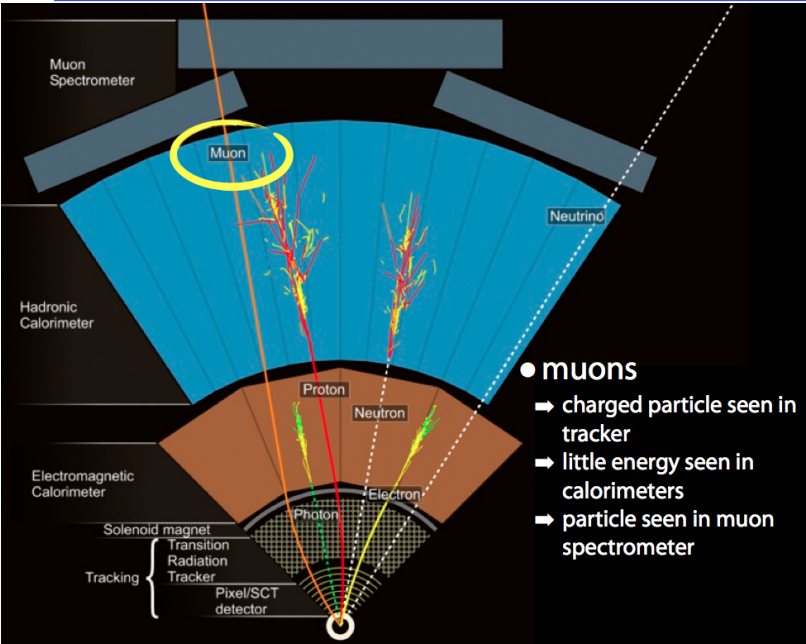
\includegraphics[scale = 0.45]{files/muon.png}}; 
 \end{tikzpicture}

\end{frame}


%hadrons + electron
\begin{frame}{\dashuline{}{\textbf{2) Semnătura pionilor, protonilor și a electronilor.}}}

 \begin{tikzpicture}[overlay, remember picture]
 \node[anchor=center, 
      xshift=0cm, 
      yshift=-0.3cm] 
     at (current page.center)
     {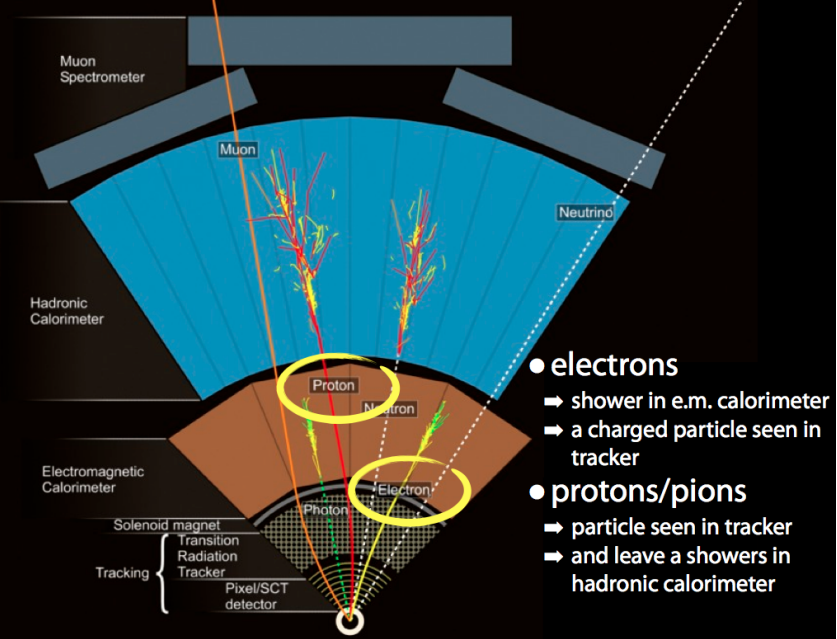
\includegraphics[scale = 0.45]{files/hadrons.png}}; 
 \end{tikzpicture}

\end{frame}

%hadrons + electron
\begin{frame}{\dashuline{}{\textbf{3) Semnăturile jeturilor de particule și ale neutrinilor.}}}

 \begin{tikzpicture}[overlay, remember picture]
 \node[anchor=center, 
      xshift=0cm, 
      yshift=-0.3cm] 
     at (current page.center)
     {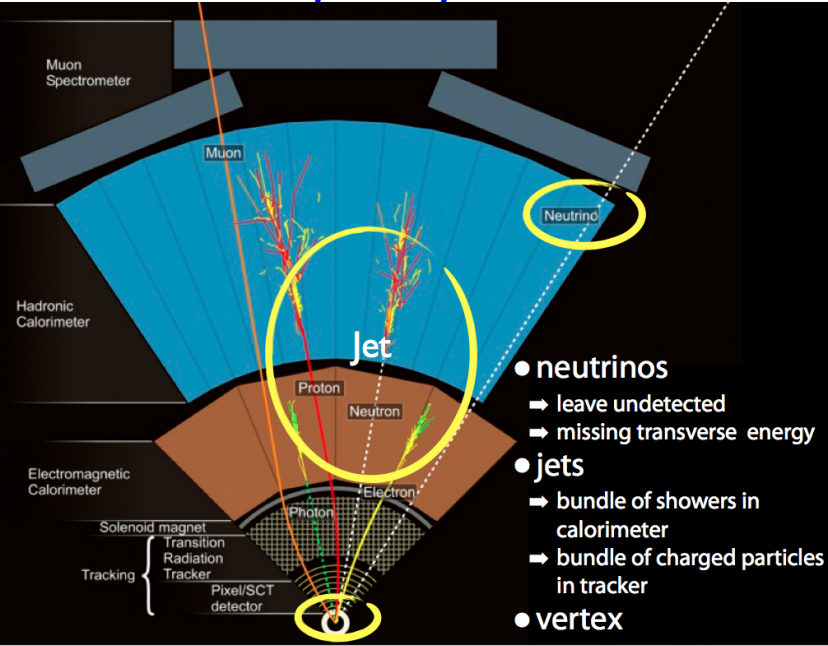
\includegraphics[scale = 0.45]{files/Jets.png}}; 
 \end{tikzpicture}

\end{frame}


%hadrons + electron
\begin{frame}{\dashuline{}{\textbf{4) Semnăturile fotonilor și ale neutronilor.}}}

 \begin{tikzpicture}[overlay, remember picture]
 \node[anchor=center, 
      xshift=0cm, 
      yshift=-0.3cm] 
     at (current page.center)
     {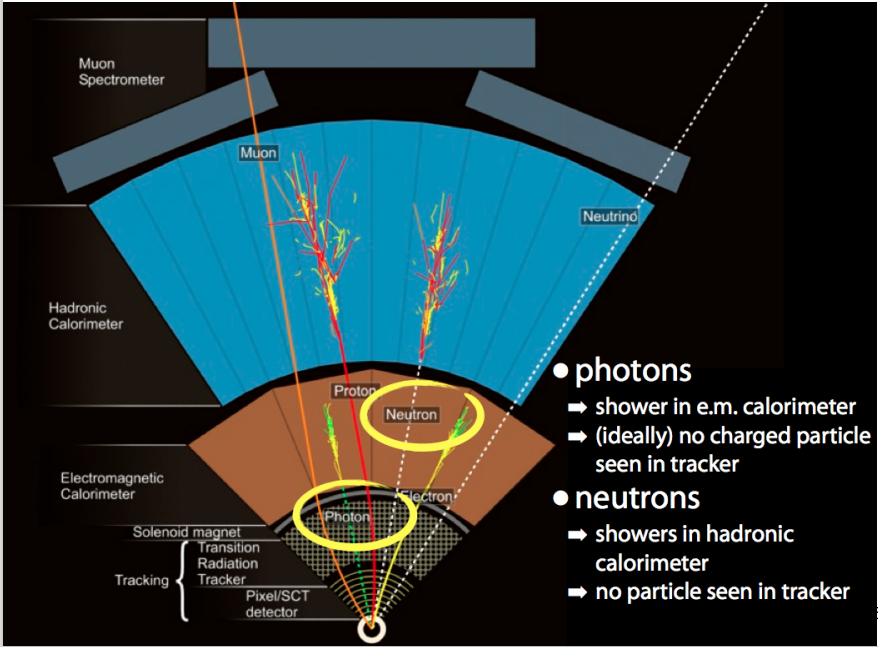
\includegraphics[scale = 0.45]{files/PhotonsNeutrons.png}}; 
 \end{tikzpicture}
\end{frame}

%%%%%%%%%%%%%%%%%%%%%%%%%%%%%%%%%%%%%%%%%%%%%%%%%%%%%%%%%%%%%%%%%5

%parametrizarea tracks-urilor

\begin{frame}

\begin{tikzpicture}[overlay, remember picture]
 \node[anchor=center, 
      xshift=0cm, 
      yshift=0cm] 
     at (current page.center)
     {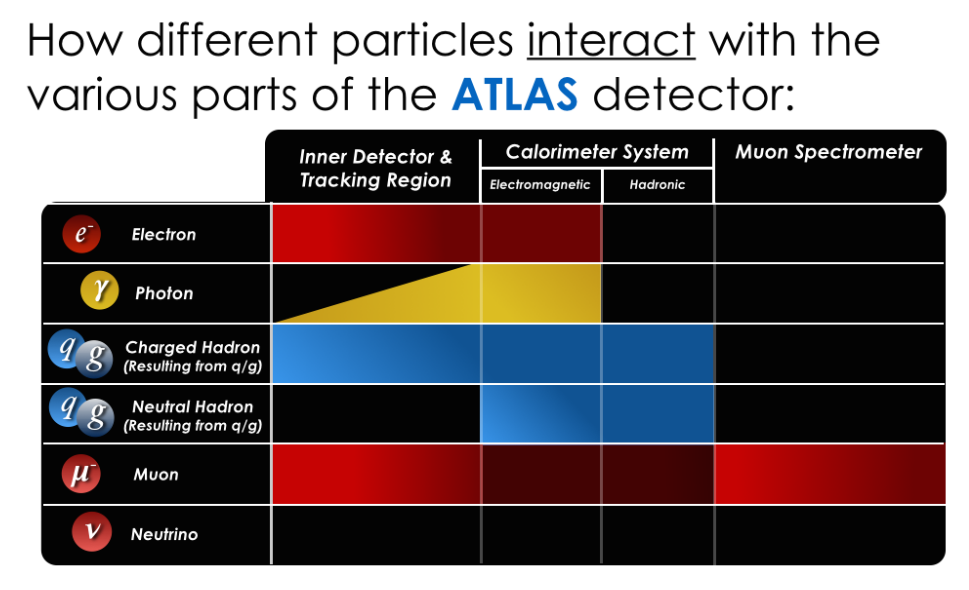
\includegraphics[scale = 0.45]{files/InteractionType.png}}; 
 \end{tikzpicture}
    
\end{frame}




\begin{frame}{\dotuline{Parametrizarea traiectoriilor particulelor.}}
\vspace{-3.3cm}
\small

\begin{itemize}

\item [\ding{99}] \makebox[0.5cm]{} \textit{\textbf{ Detectorul ATLAS colectează multe valori diferite ale parametrilor fizici. Pentru a înțelege acești parametri, este mai întâi necesar să descriem spațiul în care
au loc ciocnirile. Cea mai generală reprezentare a parametrilor este cea clasică; }}

\end{itemize}


 \begin{tikzpicture}[overlay, remember picture]
 \node[anchor=center, 
      xshift=-2.4cm, 
      yshift=0cm] 
     at (current page.center)
     {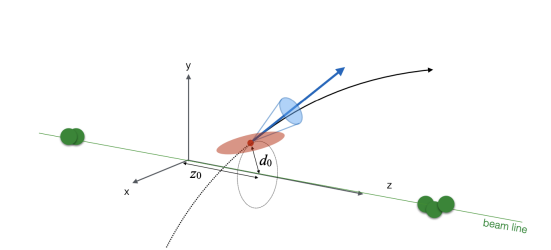
\includegraphics[scale = 0.4]{files/Parametrizarea.png}}; 
 \end{tikzpicture}

\begin{tikzpicture}[overlay, remember picture]
 \node[anchor=center, 
      xshift=-2.8cm, 
      yshift=-2.5cm] 
     at (current page.center)
     {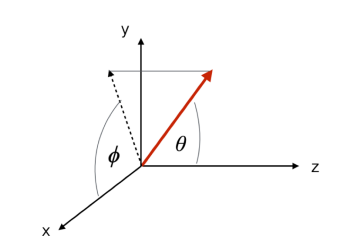
\includegraphics[scale = 0.4]{files/coordinate system.png}}; 
 \end{tikzpicture}

 \begin{tikzpicture}[overlay, remember picture]
 \node[anchor=center, 
      xshift= 2.4cm, 
      yshift=0.5cm] 
     at (current page.center)
     {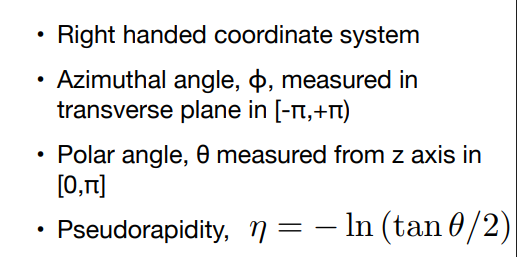
\includegraphics[scale = 0.4]{files/Param.png}}; 
 \end{tikzpicture}

 \begin{tikzpicture}[overlay, remember picture]
 \node[anchor=center, 
      xshift=2.5cm, 
      yshift=-2.5cm] 
     at (current page.center)
     {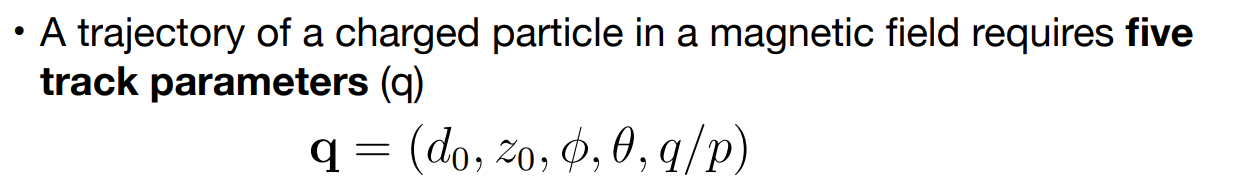
\includegraphics[scale = 0.2]{files/all param.png}}; 
 \end{tikzpicture}

\end{frame}



%alte detalii esențiale;
\begin{frame}{\textbf{Luminozitatea instantanee și cea integrată!}}

\vspace{-0cm}

\begin{itemize}
   \item \makebox[0.5cm]{} \textbf{\textit{Pentru a forma particule mai grele și mai interesante este nevoie de un număr mare de ciocniri...}}
   \item \makebox[0.5cm]{} \textbf{\textit{Luminozitatea instantanee, notată cu L, este o măsură a numărului de ciocniri care poate fi produs într-un detector pe centimetru pătrat, pe secundă.}}

   \item \makebox[0.5cm]{} \textbf{\textit{Acest parametru se definește ca fiind raportul dintre numărul de evenimente detectate în unitatea de timp și secțiunea transversală; L(t)=dN/s*dt }}

   \item \makebox[0.5cm]{} \textbf{\textit{Secțiunea transversală(s) a unei particule dă probabilitatea pentru ca o interacțiune/împrăștiere cu alte particule să aibă loc}}

   \item \makebox[0.5cm]{} \textbf{\textit{Luminozitatea integrată(Lint) este o măsură a datelor colectate pe parcursul unui "run" și se definește ca: \[ \int_{0}^{T} L(t) \,dt \]}}
\end{itemize}
    
\end{frame}


%evenimente utile
\begin{frame}{Evenimente utile}
\begin{tikzpicture}[overlay, remember picture]
 \node[anchor=center, 
      xshift=0cm, 
      yshift=1cm] 
     at (current page.center)
     {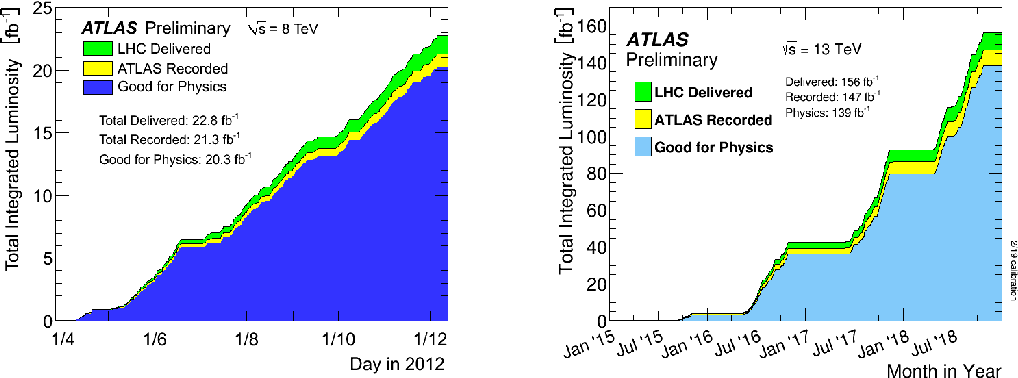
\includegraphics[scale = 0.34]{files/51-Figure25-1.png}}; 
 \end{tikzpicture}

\vspace{3.8cm}
\begin{itemize}
\small    
\item \makebox[0.5cm]{} \textbf{\textit{Femtobarnul invers nu este o măsură a informației, ci mai degrabă a eficacității acceleratorului de particule. Un femtobarn invers este echivalat cu aproximativ 70 de milioane de milioane de coliziuni înregistrate. Numărul total de coliziuni este direct proporțional cu "luminozitatea" coliziunilor măsurate în acest timp.}}



\end{itemize}   
\end{frame}




%PTE -> sau impulsul transversal lipsa
\begin{frame}{\dashuline{\textbf{Impulsul transversal lipsă(sau \textcolor{red}{ETMiss})!}}}

\vspace{0cm}

\begin{enumerate}
  \small
  \item[I] \makebox[0.5cm]{} \textbf{ Indiferent de modul în care impulsul este împărțit între constituenții unui proton, valoarea sa totală pentru fiecare proton în ansamblu trebuie să fie de ~7 TeV/c - impulsul trebuie să fie total orientat în direcția axei Oz.}

  \item[II] \makebox[0.5cm]{} Impulsul total perpendicular pe linia fasciculului este zero(într-un plan transversal), pe baza legilor de conservare! Acest fapt este de o importanță capitală în coliziunile din ATLAS.

  \item[III] \makebox[0.5cm]{} \textbf{O fracțiune de impuls transversal lipsă se rezumă direct la un dezechilibru energetic: mai multă energie măsurată pe o parte a detectorului și relativ mai puțină pe cealaltă parte.}

  \item[IV] \makebox[0.5cm]{} Deci, o cantitate mare de energie transversală lipsă sugerează prezența unei particule care nu interacționează cu detectorii dar care a transportat energia necesară echilibrului energetic.

  \item[IV] \makebox[0.5cm]{} \textbf{\textcolor{red}{Această cantitate lipsă este figurată cu o linie roșie întreruptă care, în plus față de valoarea(care este mărimea impulsului/energiei lipsă) arată direcția vectorului momentului transversal lipsă.}}
\end{enumerate}

\end{frame}



%masa invairantă 

\begin{frame}{\textbf{\dashuline{Masa invariantă.}}}

\vspace{0cm}
\begin{enumerate}
  \small
  \item[A)] \makebox[0.5cm ]{} \textit{ \textcolor{blue}{Masa invariantă se mai numește "masă de repaus" și este caracteristică oricărei particule, fiind o mărime care nu se modifică cu viteza sau cu cadrul de referință. 
 Pentru a determina masa invariantă a unei particule care se descompune aproape instantaneu, trebuie să ne uităm la produsele sale de dezintegrare. Se măsoară energia și impulsul fiecărei particule produse și apoi se însumează toate energiile acestora.}}\\
 
  \item[B)] \makebox[0.5cm]{} \textit{\textbf{Rezultatul este masa invariantă totală a reactantului iar dacă analizăm o particulă țintă, atunci masa calculată în fiecare eveniment ar trebui să fie "aproape" aceeași, așa că dacă plotăm distribuția maselor pentru diferite evenimente, vom putea vedea un maxim de rezonanță(peak) în jurul "masei medii" a particulei.}}\\

   \item[C)] \makebox[0.5cm]{} \textit{\textbf{\textcolor{magenta}{Obiectivul cheie constă în a reasambla evenimentul de la coadă la cap, pe baza caracteristicilor parametrice ale produșilor de dezintegrare specifici particulei căutate.}}}

    \item[E)] \makebox[0.5cm]{} \textit{\textbf{\dotuline{HYPATIA permite vizualizarea unui tabel cu valorile parametrilor fizici și geometrici specifici diferitelor particule.}}}
   
\end{enumerate}

\end{frame}


%YZ section
\begin{frame}{\dashuline{}{\textbf{Detectorul ATLAS în ansamblu- proiecția YZ.}}}

 \begin{tikzpicture}[overlay, remember picture]
 \node[anchor=center, 
      xshift=-2cm, 
      yshift=1.5cm] 
     at (current page.center)
     {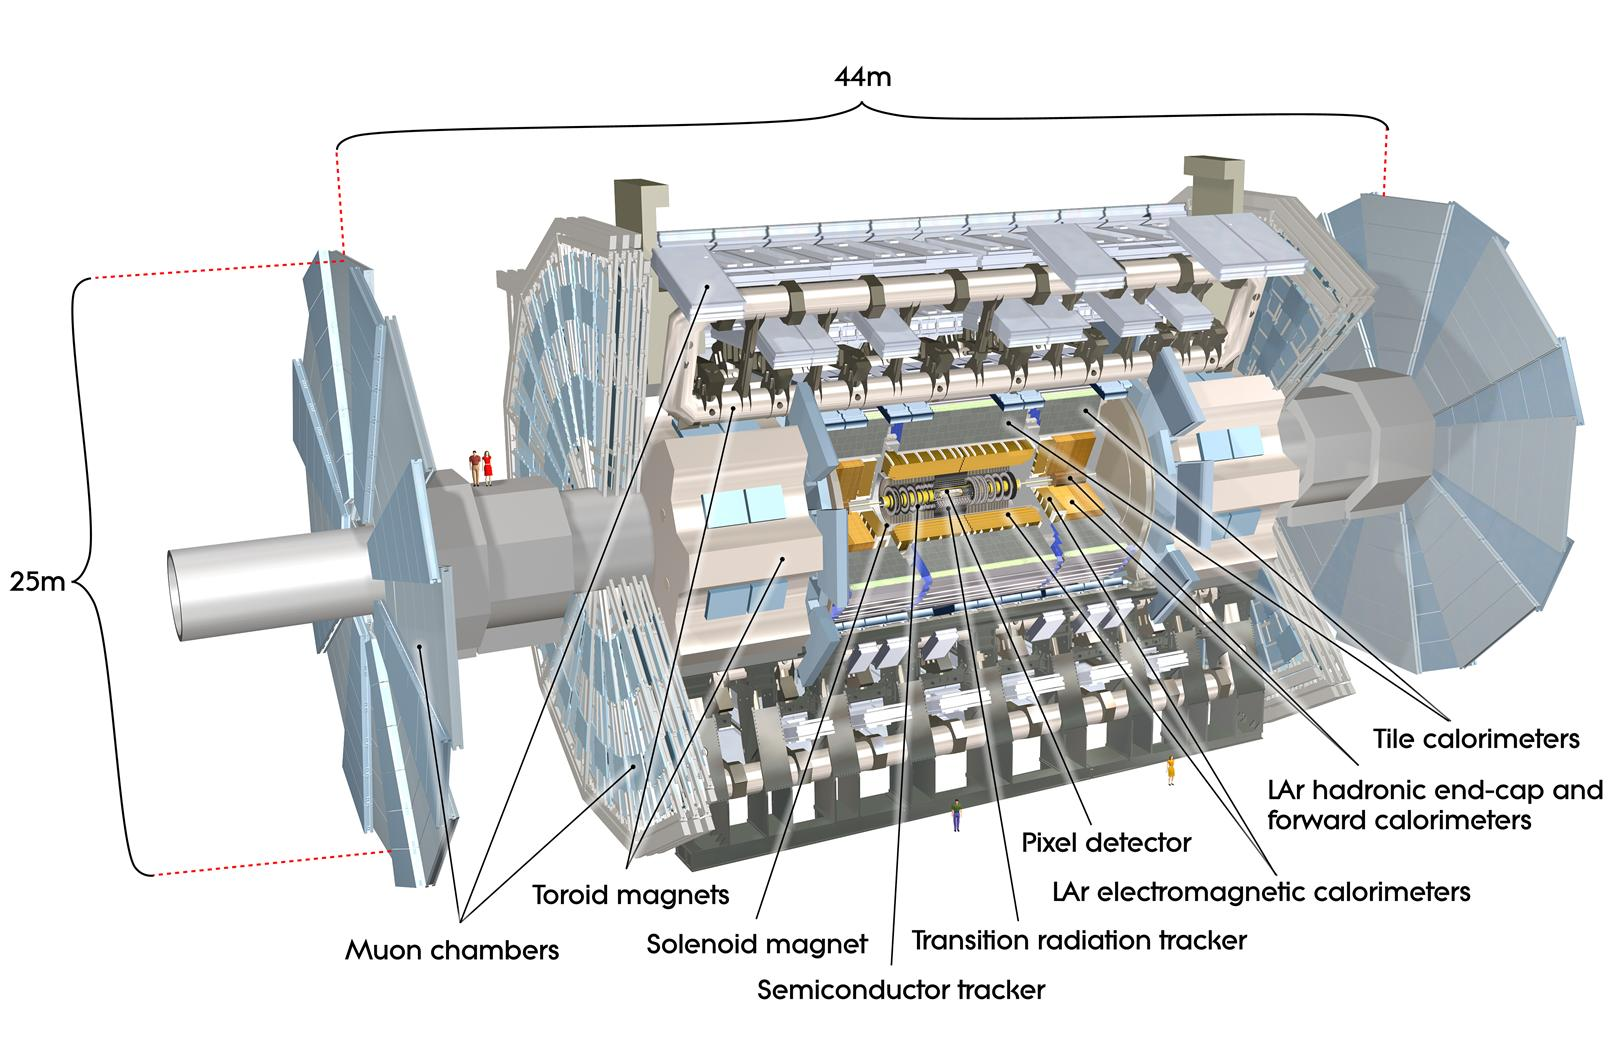
\includegraphics[scale = 0.25]{files/R.jpg}}; 
 \end{tikzpicture}

  \begin{tikzpicture}[overlay, remember picture]
 \node[anchor=center, 
      xshift=4cm, 
      yshift=1.5cm] 
     at (current page.center)
     {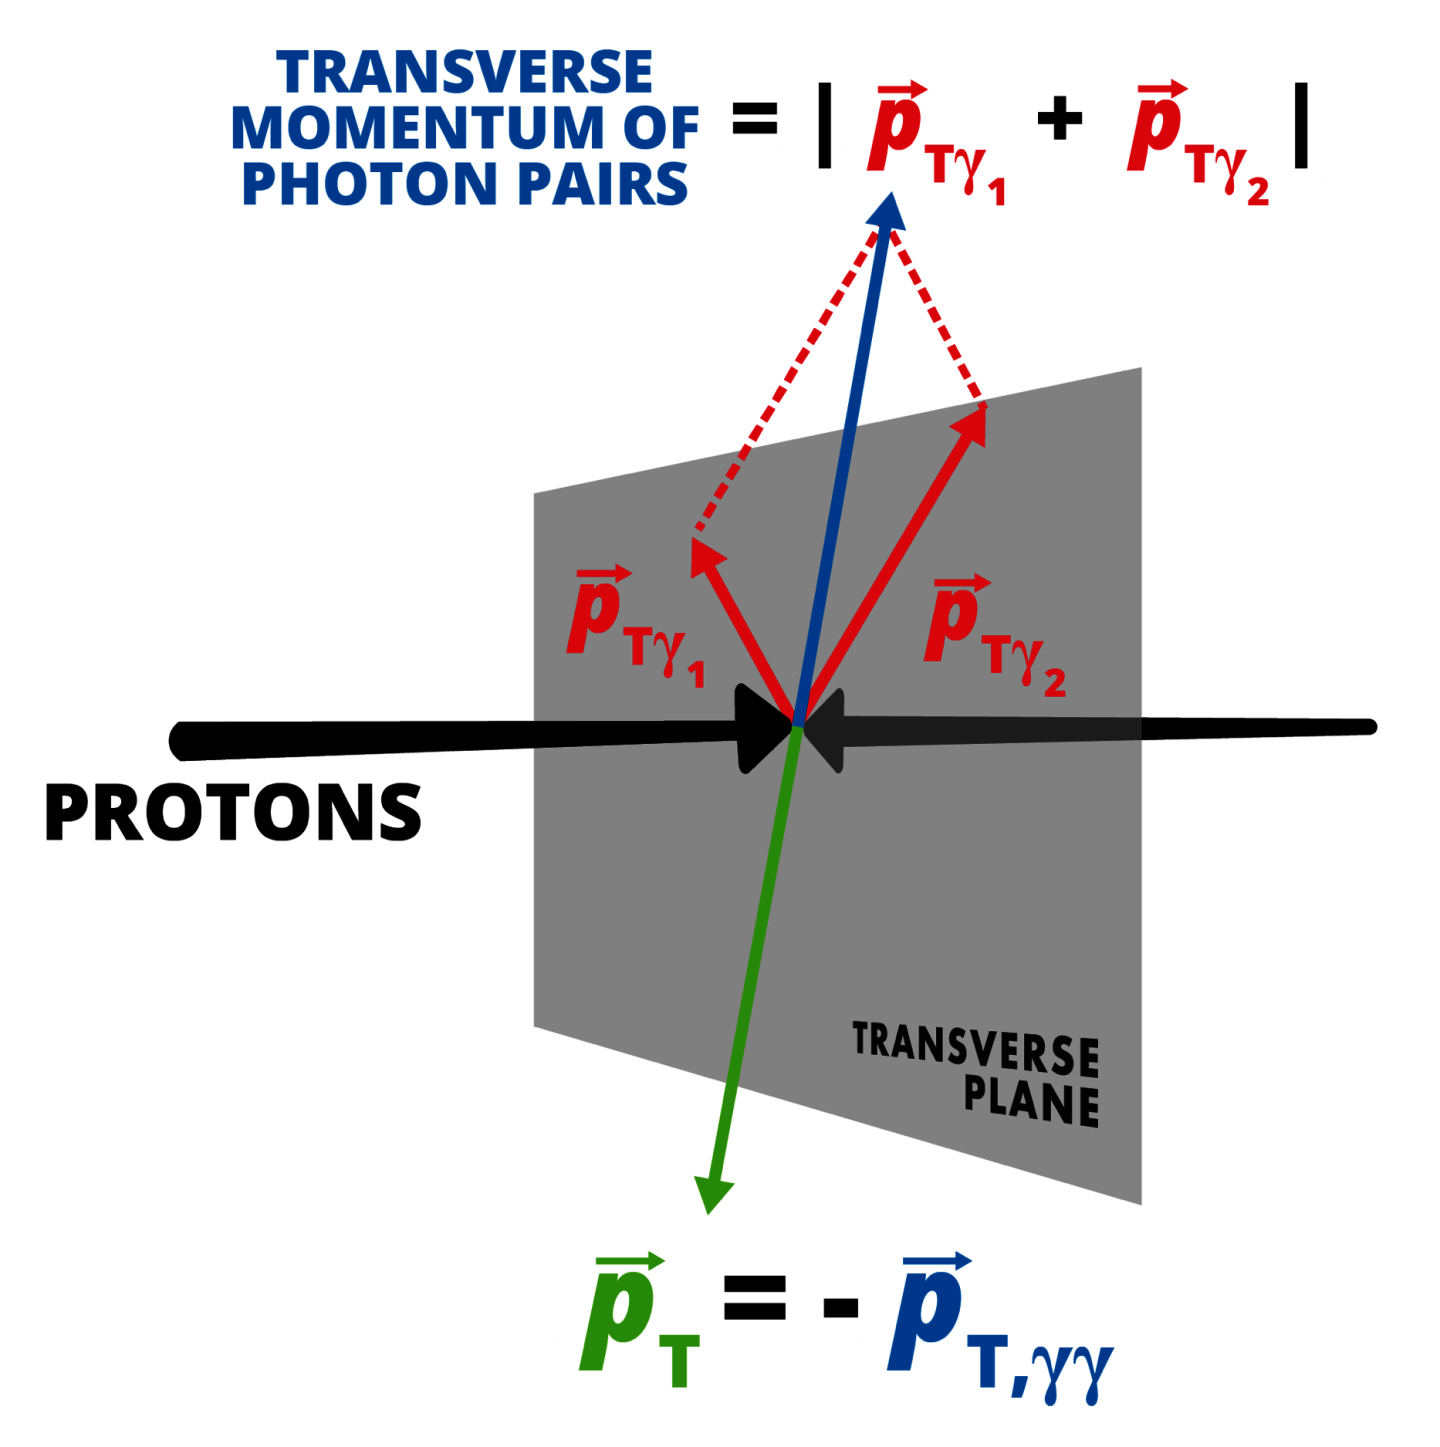
\includegraphics[scale = 0.06]{files/ATLAS-diphoton-illustration-01.png}}; 
 \end{tikzpicture}

\begin{tikzpicture}[overlay, remember picture]
 \node[anchor=center, 
      xshift=3cm, 
      yshift=-2.5cm] 
     at (current page.center)
     {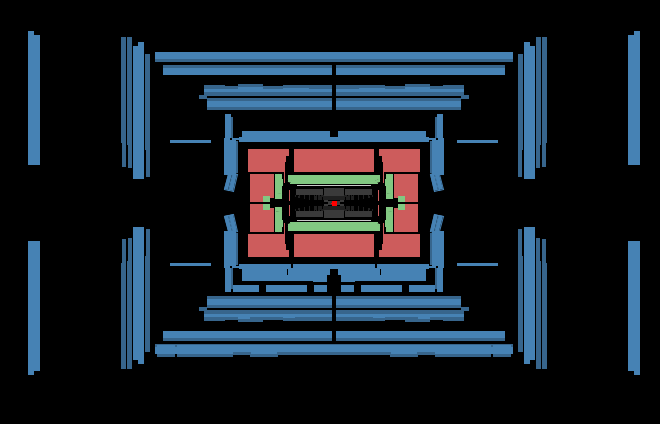
\includegraphics[scale = 0.3]{files/2-proiectia RoZ.png}}; 
 \end{tikzpicture}

\begin{tikzpicture}[overlay, remember picture]
 \node[anchor=center, 
      xshift=-3cm, 
      yshift=-2.5cm] 
     at (current page.center)
     {
\includegraphics[scale = 0.25]{files/Hypatia1.png}}; 
 \end{tikzpicture}
 
\end{frame}


%hypatia cross section
\begin{frame}{\dashuline{}{\textbf{\small Detectorul ATLAS în HYPATIA- proiecția din planul XY.}}}

 \begin{tikzpicture}[overlay, remember picture]
 \node[anchor=center, 
      xshift=-2.3cm, 
      yshift=0cm] 
     at (current page.center)
     {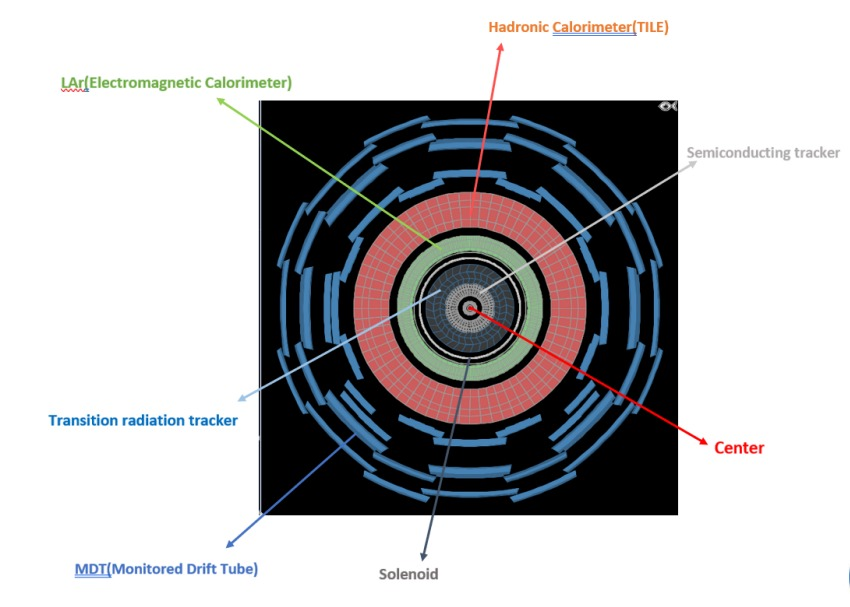
\includegraphics[scale = 0.27]{files/OnionStructure.jpeg}}; 
 \end{tikzpicture}

 \begin{tikzpicture}[overlay, remember picture]
 \node[anchor=center, 
      xshift=3.5cm, 
      yshift=-1cm] 
     at (current page.center)
     {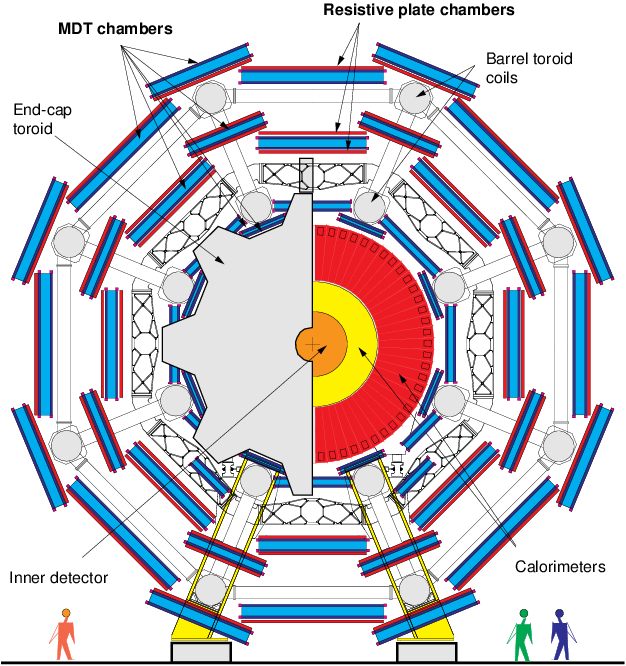
\includegraphics[scale = 0.4]{files/Cross-view-of-the-muon-spectrometer.png}}; 
 \end{tikzpicture}

 \begin{tikzpicture}[overlay, remember picture]
 \node[anchor=center, 
      xshift=-3cm, 
      yshift=-3.5cm] 
     at (current page.center)
     {
\includegraphics[scale = 0.23]{files/Hypatia1.png}}; 
 \end{tikzpicture}

\end{frame}


%hypatia interfata totala
\begin{frame}{\dashuline{}{\textbf{Cum arată HYPATIA?}}}

 \begin{tikzpicture}[overlay, remember picture]
 \node[anchor=center, 
      xshift=0cm, 
      yshift=0cm] 
     at (current page.center)
     {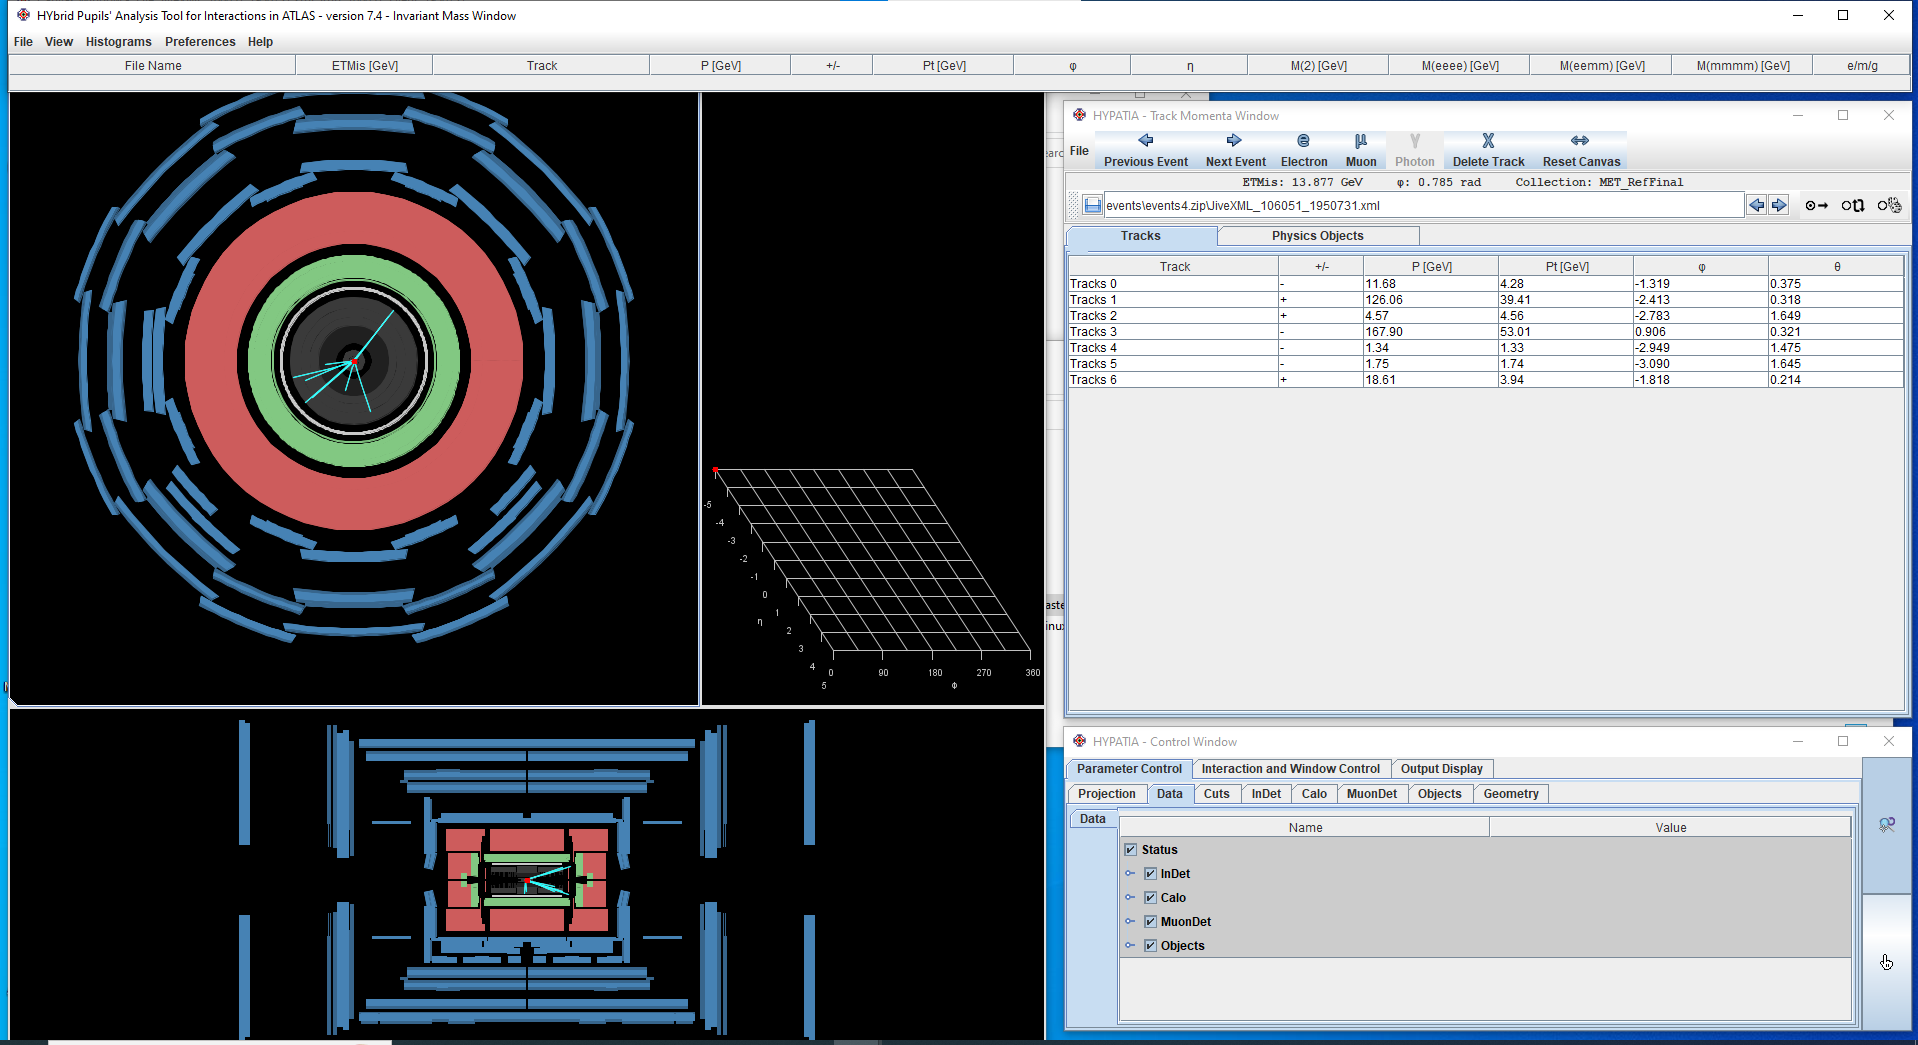
\includegraphics[scale = 0.25]{files/InterfataTot.png}}; 
 \end{tikzpicture}
 \end{frame} 


%ce ne permite softul:

\begin{frame}{\textbf{\dashuline{Ce ne permite softul pentru o analiză certă?}}}

\vspace{0cm}
\begin{enumerate}
  \small
  \item[a)] \makebox[0.5cm ]{} \textbf{\textit{ \textcolor{blue}{Calculul automat precum și exportarea maselor invariante pentru anumite perechi compatibile de particule(din tabelul Invariant Mass Window), spre exemplu electron-pozitron, muon-antimuon.}}}\\
 
  \item[b)] \makebox[0.5cm]{} \textit{\textbf{\textcolor{red}{Vizualizarea direcției impulsului transversal lipsă(linia roșie, punctată) - cât și afișarea valorii energiei transversale lipsă! }}}\\

   \item[c)] \makebox[0.5cm]{} \textit{\textbf{\textcolor{green}{Setarea unor filtre energetice pentru afișarea selectivă a evenimentelor, filtre care sunt de altfel condiții de constrângere după anumite criterii.}}}

    \item[d)] \makebox[0.5cm]{} \textit{\textbf{Contabilizarea numărului de lovituri(numPixelHits, numSCTHits, numTRTHits)  în fiecare parte a detectorului interior, funcție de tracks(semnătura particulei).}}

    \item[e)] \makebox[0.5cm]{} \textit{\textbf{\textcolor{gray}{Evaluarea depozitelor energetice în calorimetre(și reprezentarea lor în diagrama lego) + afișarea jeturilor de particule sau chiar a unor particule compozite.}}}

\end{enumerate}

\end{frame}

%hypatia - filtrul1
\begin{frame}{\dashuline{}{\textbf{Filter1 - InnerDetector:}}}

 \begin{tikzpicture}[overlay, remember picture]
 \node[anchor=center, 
      xshift=0cm, 
      yshift=0cm] 
     at (current page.center)
     {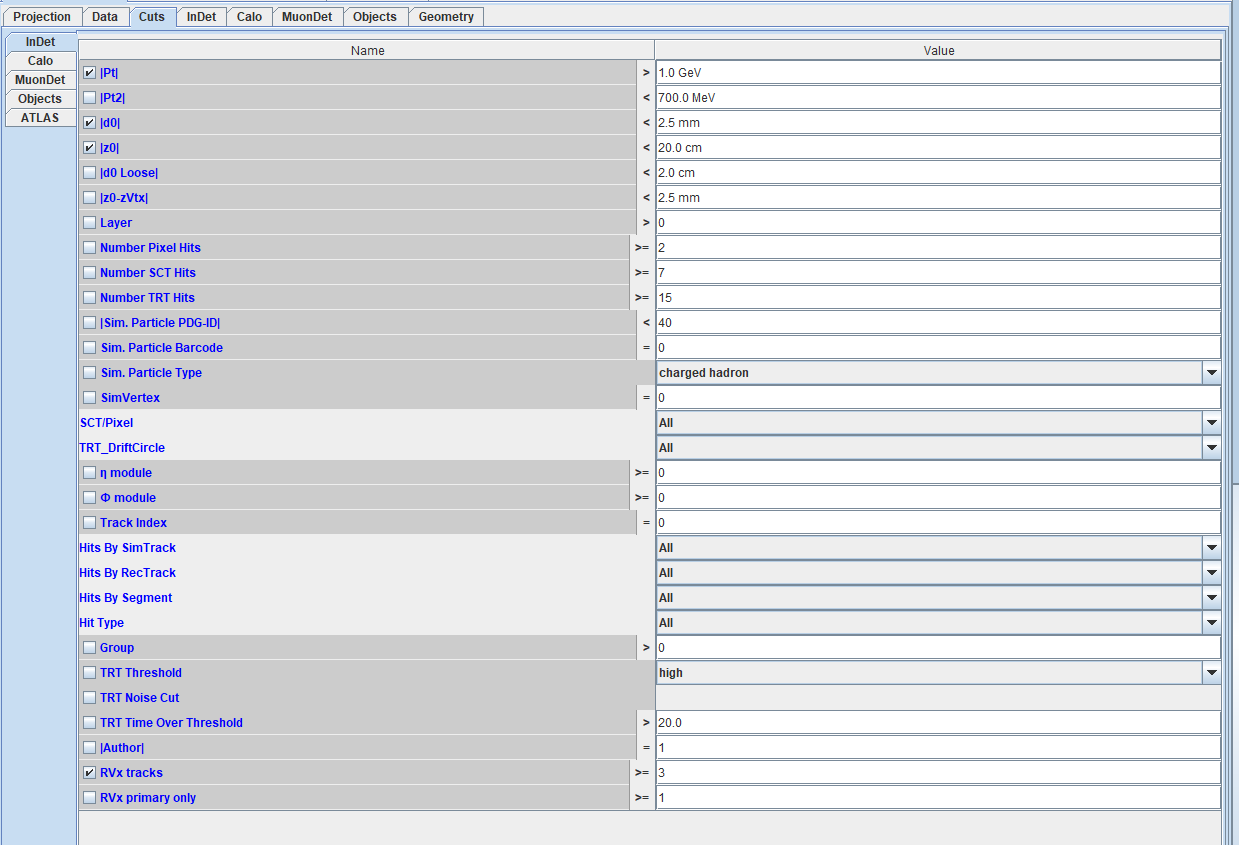
\includegraphics[scale = 0.33]{files/Cuts Filter.png}}; 
 \end{tikzpicture}
 \end{frame} 

 %hypatia - filtrul2
\begin{frame}{\dashuline{}{\textbf{Filter2 - Calorimeters:}}}

 \begin{tikzpicture}[overlay, remember picture]
 \node[anchor=center, 
      xshift=0cm, 
      yshift=0cm] 
     at (current page.center)
     {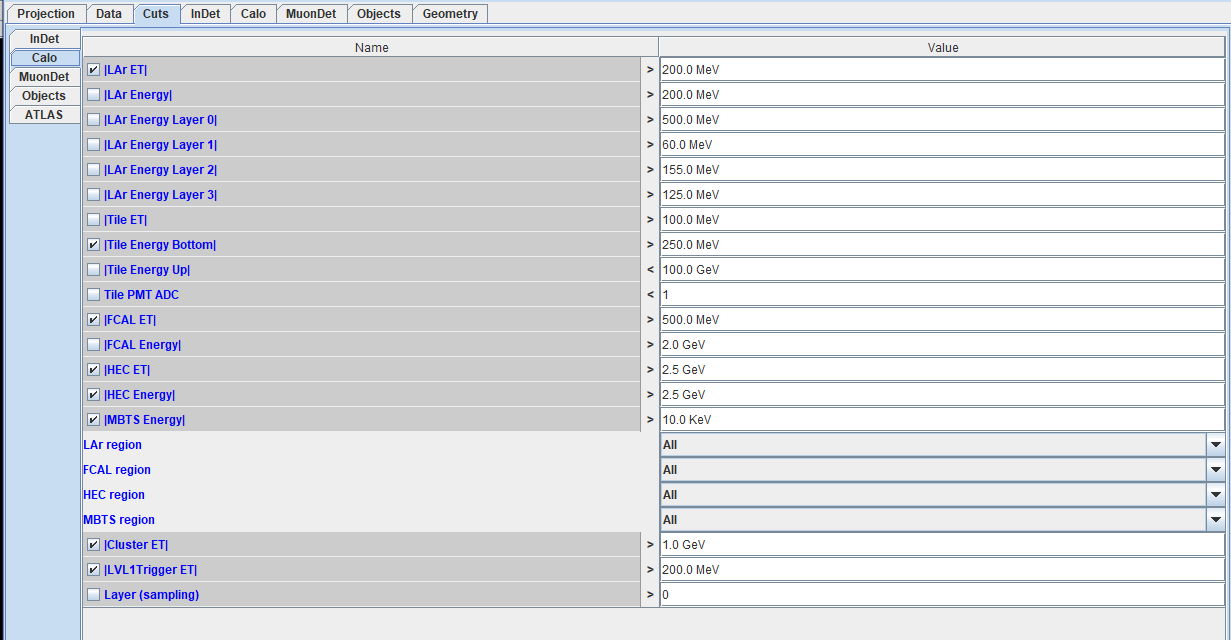
\includegraphics[scale = 0.35]{files/Cuts Filter 2.png}}; 
 \end{tikzpicture}
 \end{frame} 

  %hypatia - filtrul3 
\begin{frame}{\dashuline{}{\textbf{Filter2 - Objects:}}}

 \begin{tikzpicture}[overlay, remember picture]
 \node[anchor=center, 
      xshift=0cm, 
      yshift=0cm] 
     at (current page.center)
     {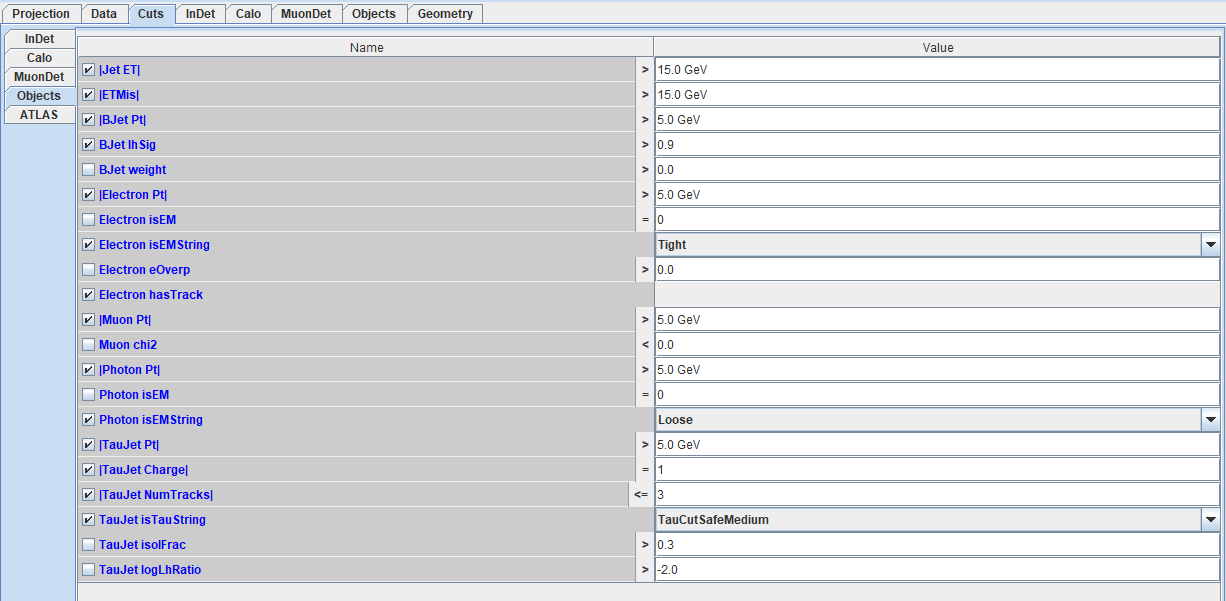
\includegraphics[scale = 0.37]{files/Cuts Filter 3.png}}; 
 \end{tikzpicture}
 \end{frame} 


   %hypatia - Depozit energetic 
\begin{frame}{\dashuline{}{\textbf{Depozit Energetic în LAr - Output Display:}}}

 \begin{tikzpicture}[overlay, remember picture]
 \node[anchor=center, 
      xshift=0cm, 
      yshift=-0.5cm] 
     at (current page.center)
     {\includegraphics[scale = 0.35]{files/DepozitEnergetic.png}}; 
 \end{tikzpicture}
 
 \end{frame} 


%Jets
\begin{frame}{\dashuline{}{\textbf{Jeturi de particule - asociate cu depozite energetice:}}}

 \begin{tikzpicture}[overlay, remember picture]
 \node[anchor=center, 
      xshift=0cm, 
      yshift=-0.5cm] 
     at (current page.center)
     {\includegraphics[scale = 0.4]{files/Jet1.png}}; 
 \end{tikzpicture}
 
 \end{frame} 


%Detectarea varfurilor sau rezonantelor;

\begin{frame}{\dashuline{}{\textbf{General Objects:}}}

 \begin{tikzpicture}[overlay, remember picture]
 \node[anchor=center, 
      xshift=0cm, 
      yshift=0cm] 
     at (current page.center)
     {\includegraphics[scale = 0.4]{files/AtlasObjects.png}}; 
 \end{tikzpicture}

 \end{frame}

 %ce am reușit.

\begin{frame}{\dashuline{}{\textbf{\underline{Ce avem de făcut?}}}}

\vspace{0cm}
\begin{enumerate}
  \small
  \item[1)] \makebox[0.5cm ]{} \textbf{\textit{ \textcolor{black}{Trebuie să reperăm perechi de particule care îndeplinesc anumite criterii energetice - spre a putea reconstitui(indirect) anumite canale de dezintegrare specifice unor particule cu un timp foarte scurt de viață.}}}\\
 
  \item[2)] \makebox[0.5cm]{} \textit{\textbf{\textcolor{black}{Să impunem un criteriu de selecție destul de ferm: ca impulsul transversal al particulelor rezultate din eveniment să fie strict mai mare decât o valoare critică minimă (20 GeV/c)! }}}\\

  \item[3)] \makebox[0.5cm]{} \textit{\textbf{\textcolor{black}{Să grupăm în perechi diferite pariticule: pentru a putea repera, pe baza maselor lor invariante, reactantul original! }}}\\

  \item[4)] \makebox[0.5cm]{} \textit{\textbf{\textcolor{black}{Să reprezentăm o distribuție invariantă de tip histogramă care să arate dependența numărului de evenimente funcție de energia lor medie pe anumite regiuni! }}}\\

  \item[5)] \makebox[0.5cm]{} \textit{\textbf{\textcolor{black}{Să identificăm pe baza graficului acele maxime/rezonanțe care corespund unor valori masice remarcabile; pe seama acestor "peak-uri" se vor aprecia particulele rare care au fost produse. }}}\\

\end{enumerate}

\end{frame} 



% Descriere detaliata
\begin{frame}{\dashuline{}{\textbf{Detalii de substrat:}}}

 \begin{tikzpicture}[overlay, remember picture]
 \node[anchor=center, 
      xshift=-2cm, 
      yshift=2cm] 
     at (current page.center)
     {\includegraphics[scale = 0.5]{files/WhatToDo.png}}; 
 \end{tikzpicture}

 \begin{tikzpicture}[overlay, remember picture]
 \node[anchor=center, 
      xshift=-3cm, 
      yshift=-2cm] 
     at (current page.center)
     {\includegraphics[scale = 0.35]{files/Reconstruction.png}}; 
 \end{tikzpicture}

 \begin{tikzpicture}[overlay, remember picture]
 \node[anchor=center, 
      xshift=2.7cm, 
      yshift=-3cm] 
     at (current page.center)
     {\includegraphics[scale = 0.45]{files/Mixture.png}}; 
 \end{tikzpicture}

 \end{frame} 

 
%Histograma mea
\begin{frame}{\dashuline{}{\textbf{Histograma obținută de noi:}}}

 \begin{tikzpicture}[overlay, remember picture]
 \node[anchor=center, 
      xshift=0cm, 
      yshift=0cm] 
     at (current page.center)
     {\includegraphics[scale = 0.4]{files/DiLeptHisto.png}}; 
 \end{tikzpicture}

\end{frame}

%explicatia rezonantelor
\begin{frame}{\dashuline{}{\textbf{\underline{Ce am dedus?}}}}

\vspace{0cm}
\begin{enumerate}
  \small
  \item \makebox[0.5cm ]{} \textbf{\textit{ \textcolor{blue}{În graficul precedent am observat care este distribuția numărului de evenimente di-leptonice(de tipul electron-pozitron sau muon-antimuon) funcție de masa invariantă medie. }}}\\
 
  \item \makebox[0.5cm]{} \textit{\textbf{\textcolor{blue}{Această distribuție statistică se numește distribuție de masă invariantă și pentru o scală logaritmică a axei Ox ea primite dezvăluirea unor concentrări/maxime numite uzual rezonanțe.}}}\\

  \item \makebox[0.5cm]{} \textit{\textbf{\textcolor{blue}{De notat este că am putut evidenția simultan cca. 4 rezonanțe sau peak-uri aferente unor bosoni: 
  Z(~90 GeV), Z’(~1000 GeV), $\Upsilon$(~10 GeV) și J/$\psi$(~3 GeV). Aceste particule au canale de dezintegrare di-leptonice !}}}\\

  \item \makebox[0.5cm]{} \textit{\textbf{\textcolor{blue}{Au fost utilizate doar câteva sute de evenimente! Distribuția este cu mult mai fină pentru un număr superior de evenimente. }}}\\
   ................................................................................................
  \item \makebox[0.5cm]{} \textit{\textbf{\textcolor{black}{În următorul slide se regăsește un alt exemplu care înfățișează aceste maxime cu o mai bună precizie- pentru o mulțime mai mare de date colectate. }}}\\

\end{enumerate}

\end{frame} 


% diagrama finala
\begin{frame}{\dashuline{}{\textbf{Pentru câteva mii de evenimente combinate:}}}

 \begin{tikzpicture}[overlay, remember picture]
 \node[anchor=center, 
      xshift=0cm, 
      yshift=0cm] 
     at (current page.center)
     {\includegraphics[scale = 0.6]{files/PlotDemons.png}}; 
 \end{tikzpicture}

 \vspace{5.5cm}
 
\begin{enumerate}
  \small
\item \makebox[0.5cm ]{} \textbf{\textit{ \textcolor{red}{Aceste semnale utile sunt decisive în identificarea bosonilor căutați. }}}\\
  \end{enumerate}

 \end{frame}


%3 alte distribuții de mase invariante:
 \begin{frame}{\dashuline{}{\textbf{Alte distribuții invariante:}}}

 \begin{tikzpicture}[overlay, remember picture]
 \node[anchor=center, 
      xshift=0cm, 
      yshift=0.2cm] 
     at (current page.center)
     {\includegraphics[scale = 0.35]{files/EXPECTED_ALL_OTHER.png}}; 
 \end{tikzpicture}

 \vspace{5.6cm}
\begin{itemize}
  \small
    \item \makebox[0.5cm ]{} \textbf{\textit{ \textcolor{red}{Putem constata chiar și prezența unor evenimente din care au rezultat doi fotoni gamma sau două perechi di-leptonice ... \underline{BOSONUL HIGGS}!}}}\\
 \end{itemize}

 \end{frame}


%bosonul Higgs - 4l channel
 \begin{frame}{\dashuline{}{\textbf{*Identificarea Bosonului Higgs: canalul 4l}}}

 \begin{tikzpicture}[overlay, remember picture]
 \node[anchor=center, 
      xshift=0cm, 
      yshift=0.5cm] 
     at (current page.center)
     {\includegraphics[scale = 0.5]{files/4lepton.png}}; 
 \end{tikzpicture}



 \end{frame}


%my 4l histogram - data
  \begin{frame}{{\textbf{\underline{*Canalul 4l - din datele mele!}}}}

 \begin{tikzpicture}[overlay, remember picture]
 \node[anchor=center, 
      xshift=0cm, 
      yshift=0.5cm] 
     at (current page.center)
     {\includegraphics[scale = 0.35]{files/EXPECTED_4L.png}}; 
 \end{tikzpicture}

\vspace{5cm}
 \small
 \makebox[0.5cm ]{} \textbf{\textit{ \textcolor{red}{ Se vede clar că în jurul valorii de 120 GeV există un peak - înseamnă că am identificat bosonul Higgs prin acest canal de dezintegrare. }}}\\

 \end{frame}


 %bosonul Higgs
 \begin{frame}{\dashuline{{\textbf{Mecanismul Higgs $\gamma$ $\gamma$ - o altă ilustrare!}}}}

 \begin{tikzpicture}[overlay, remember picture]
 \node[anchor=center, 
      xshift=0cm, 
      yshift=0cm] 
     at (current page.center)
     {\includegraphics[scale = 0.45]{files/FF.png}}; 
 \end{tikzpicture}


 \end{frame}


%bosonul 
 \begin{frame}{\dashuline{}{\textbf{\underline{*Bosonul Higgs: mecanismul $\gamma$ $\gamma$ - datele mele!}}}}

 \begin{tikzpicture}[overlay, remember picture]
 \node[anchor=center, 
      xshift=0cm, 
      yshift=0.5cm] 
     at (current page.center)
     {\includegraphics[scale = 0.33]{files/ExpectedProbability_Higgs.png}}; 
 \end{tikzpicture}

 \vspace{5.5cm}
 
 \small
 \makebox[0.5cm ]{} \textbf{\textit{ \textcolor{red}{ - Prin procesarea a cca. 25 de evenimente pe femtobarn de secțiune eficace(în cadrul acestor date cumulate), se va observa un semnal specific în jurul valorii de 125 GeV, exact cel așteptat pentru confirmarea bosonului Higgs! }}}\\


 \end{frame}


 %Higgs channels

 \begin{frame}{\dashuline{}{\textbf{\underline{Ponderea canalelor de dezintegrare- Higgs}}}}

 \begin{tikzpicture}[overlay, remember picture]
 \node[anchor=center, 
      xshift=2cm, 
      yshift=1cm] 
     at (current page.center)
     {\includegraphics[scale = 0.4]{files/Higgs.png}}; 
 \end{tikzpicture}


 \begin{tikzpicture}[overlay, remember picture]
 \node[anchor=center, 
      xshift=-3.5cm, 
      yshift=1cm] 
     at (current page.center)
     {\includegraphics[scale = 0.2]{files/HiggsMasses.png}}; 
 \end{tikzpicture}

  \vspace{4cm}
\begin{itemize}
  \small
    \item \makebox[0.5cm ]{} \textbf{\textit{ \textcolor{violet}{Există o paletă largă de mase asociate unor bosoni Higgs(clasă de bosoni) și chiar mult mai multe canale de dezintegrare - o parte din ele au fost identificate!  }}}\\
 \end{itemize}
 
\end{frame}


% final slide
\begin{frame}{\dashuline{}{\textbf{\underline{Alte Histograme corespunzătoare! }}}}

 \begin{tikzpicture}[overlay, remember picture]
 \node[anchor=center, 
      xshift=3.5cm, 
      yshift=1cm] 
     at (current page.center)
     {\includegraphics[scale = 0.25]{files/MT_SpluB.png}}; 
 \end{tikzpicture}


 \begin{tikzpicture}[overlay, remember picture]
 \node[anchor=center, 
      xshift=-3cm, 
      yshift=1cm] 
     at (current page.center)
     {\includegraphics[scale = 0.27]{files/440482_1_En_16_Fig37_HTML.png}}; 
 \end{tikzpicture}

  \vspace{4cm}
\begin{itemize}
  \small
    \item[\ding{45}] \makebox[0.5cm]{} \textbf{\textit{ \textcolor{violet}{  Aceste grafice urmăresc ponderea sau numărul evenimentelor de un anumit tip care sunt asociate obținerii unor mase invariante - specifice bosonului Higgs și în acord cu anumite canale mai generale. }}}\\
 \end{itemize}
 
\end{frame}


% Standard Model
\begin{frame}{\dashuline{}{\textbf{\underline{Modelul Standard!}}}}

 \begin{tikzpicture}[overlay, remember picture]
 \node[anchor=center, 
      xshift=0cm, 
      yshift=-0.25cm] 
     at (current page.center)
     {\includegraphics[scale = 0.15]{files/2000px-Standard_Model_of_Elementary_Particles.svg_.jpg}}; 
 \end{tikzpicture}

 
\end{frame}


% Standard Model
\begin{frame}{\dashuline{}{\textbf{\underline{Final!}}}}

 \begin{tikzpicture}[overlay, remember picture]
 \node[anchor=center, 
      xshift=0cm, 
      yshift=0cm] 
     at (current page.center)
     {\includegraphics[scale = 0.3]{files/ATLAS13TeVOpenData.png}}; 
 \end{tikzpicture}


 
\end{frame}


\end{document}
% =============================================================
% =========================== END =============================
% =============================================================

